\documentclass{article}  
\usepackage{graphicx}
\usepackage[utf8]{inputenc}
\usepackage[T1]{fontenc}
\usepackage{float}
\usepackage[italian]{babel}
\usepackage{listings}
\usepackage[usenames]{color}
\usepackage{natbib}
\usepackage{siunitx}
\usepackage[strict]{changepage}
\usepackage{physics}
\usepackage{wrapfig}
\usepackage[a4paper, top=2cm, bottom=2cm, right=2cm, left=2cm]{geometry}
\usepackage{array}
\usepackage{color}
\usepackage{colortbl}
\usepackage{amsmath}
\usepackage{amssymb}
\usepackage{multirow}
\usepackage{enumitem}
\usepackage{hyperref}
\usepackage{times}
\usepackage{booktabs}



\title{Relazione di laboratorio: studio di catena elettronica}
\author{Docente: dott. Garfagnini, dott. Lunardon \\
Gruppo 14}
\date{Anno accademico 2019/20}

\begin{document}



\maketitle

\begin{itemize}
    \item[$\circ$] Aidin Attar - 1170698 - aidin.attar@studenti.unipd.it
    \item[$\circ$] Ema Baci - 1171107 – ema.baci@studenti.unipd.it
    \item[$\circ$] Alessandro Bianchetti – 1162147 – alessandro.bianchetti@studenti.unipd.it
\end{itemize}

\vspace{3 cm}
\begin{large}\textsc{\textbf{Scopo dell'esperienza}: studio della curva di trasferimento di un amplificatore invertente, del circuito con amplificatore delle differenze (non invertente), dei circuiti sommatore invertente, derivatore, raddrizzatore di precisione.} 
\end{large}
\vspace{8.5cm}

\begin{figure}[H]
\centering

\includegraphics[scale=0.5, angle=0]{unipd_logo.png}
\end{figure}

%\newpage \tableofcontents \newpage

\twocolumn

\subsection*{Descrizione dell'apparato} La seguente esperienza è stata svolta sul banco di lavoro 1. L'apparato di misura consiste di 
un oscilloscopio digitale Tektronix TBS 1102B EDU, un generatore di funzioni Tektronix AFG 1022, un alimentatore di tensione continua stabilizzato,
due multimetri digitali (metrix e ) e una scheda Arduino Due. 
Si è inoltre fatto uso di due integrati TL082C contenenti in tutto 4 amplificatori operazionali.

I circuiti studiati sono stati costruiti sulla basetta millefori alimentando gli amplificatori operazionali come nello schema riportato 
in figura \ref{fig:alimentazione}, in particolare si è fatto uso del modello TL082 JFET; dopodiché si sono 
costruiti i circuiti da studiare;  i valori misurati di resistenze e capacità utilizzate verranno riportati in seguito.
Si è inoltre fatto uso di due sonde con fattore di attenuazione 10x precedentemente compensate per la visualizzazione del 
segnale nei due canali dell'oscilloscopio.

Per l'analisi dati sono stati utilizzati programmi scritti in c++, root, gnuplot ed Excel.

\begin{center}
\begin{figure}[H]
\centering
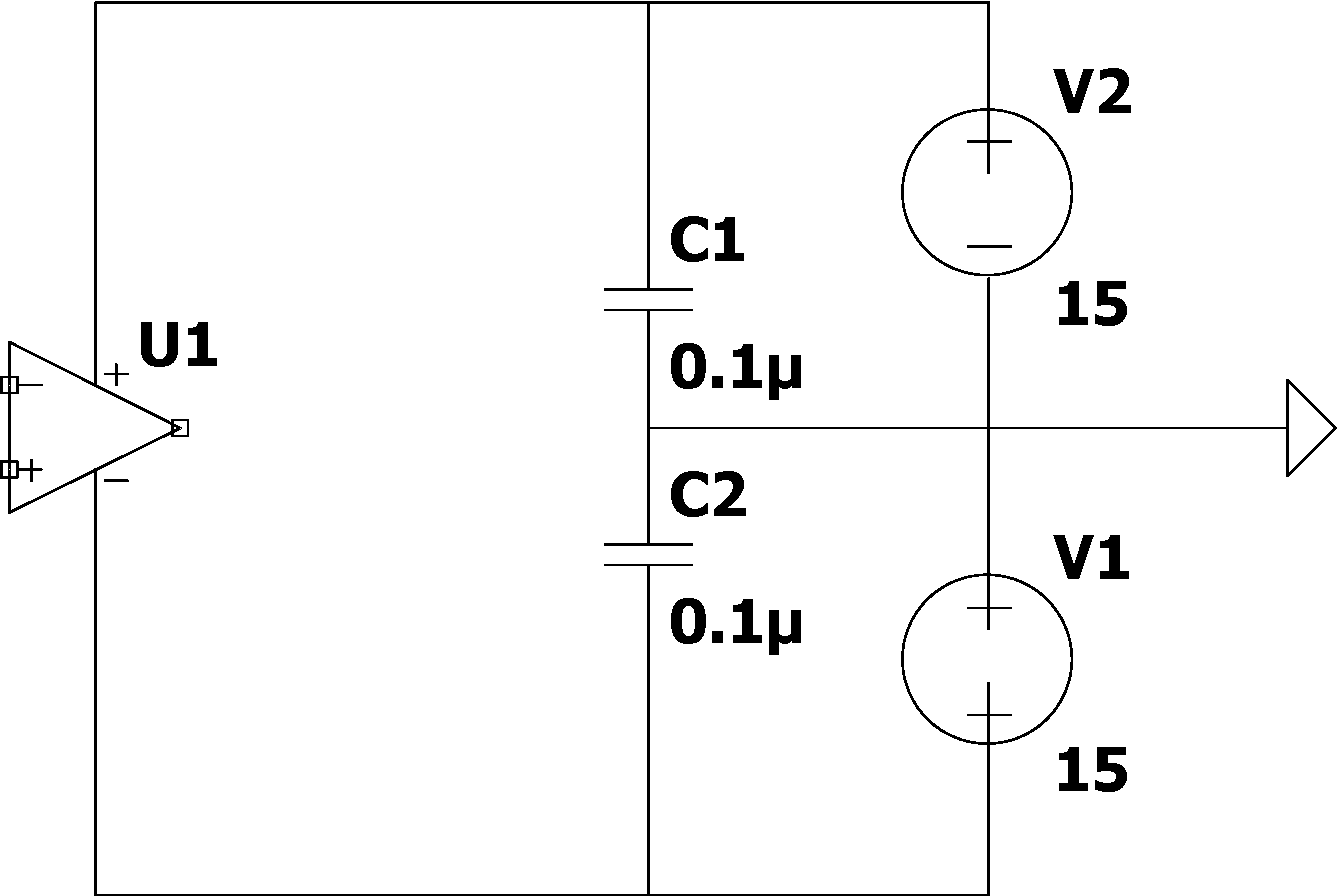
\includegraphics[scale=0.28, angle=0]{alimentazione.pdf}
\caption{ Schema per l'alimentazione dell'operazionale }
\label{fig:alimentazione}
\end{figure}
\end{center} 

\section{Preamplificatore di carica}

\subsection{Breve discussione del circuito}

Lo scopo dell'esperienza completa è costruire un circuito che possa rilevare piccoli segnali, amplificarli tanto da poterli processare con più facilità
e poi amplificarli ulteriormente per offrirli allo sperimentatore. Il primo passo della realizzazione di tale \textit{catena elettronica} è il circuito
preamplificatore. Qui il generatore di funzione è utilizzato proprio per simulare piccoli segnali di cui sopra analoghi a quelli che proverrebbero tipicamente 
da esperienze di spettrocopia: si forniscono dunque in ingresso impulsi di tensione (PULSE) come quelli che produrrebbe il passaggio di una radiazione ionizzante in 
un volume di gas. 
Si è dunque costruito il circuito come in figura

\begin{center}
\begin{figure}[H]
\centering
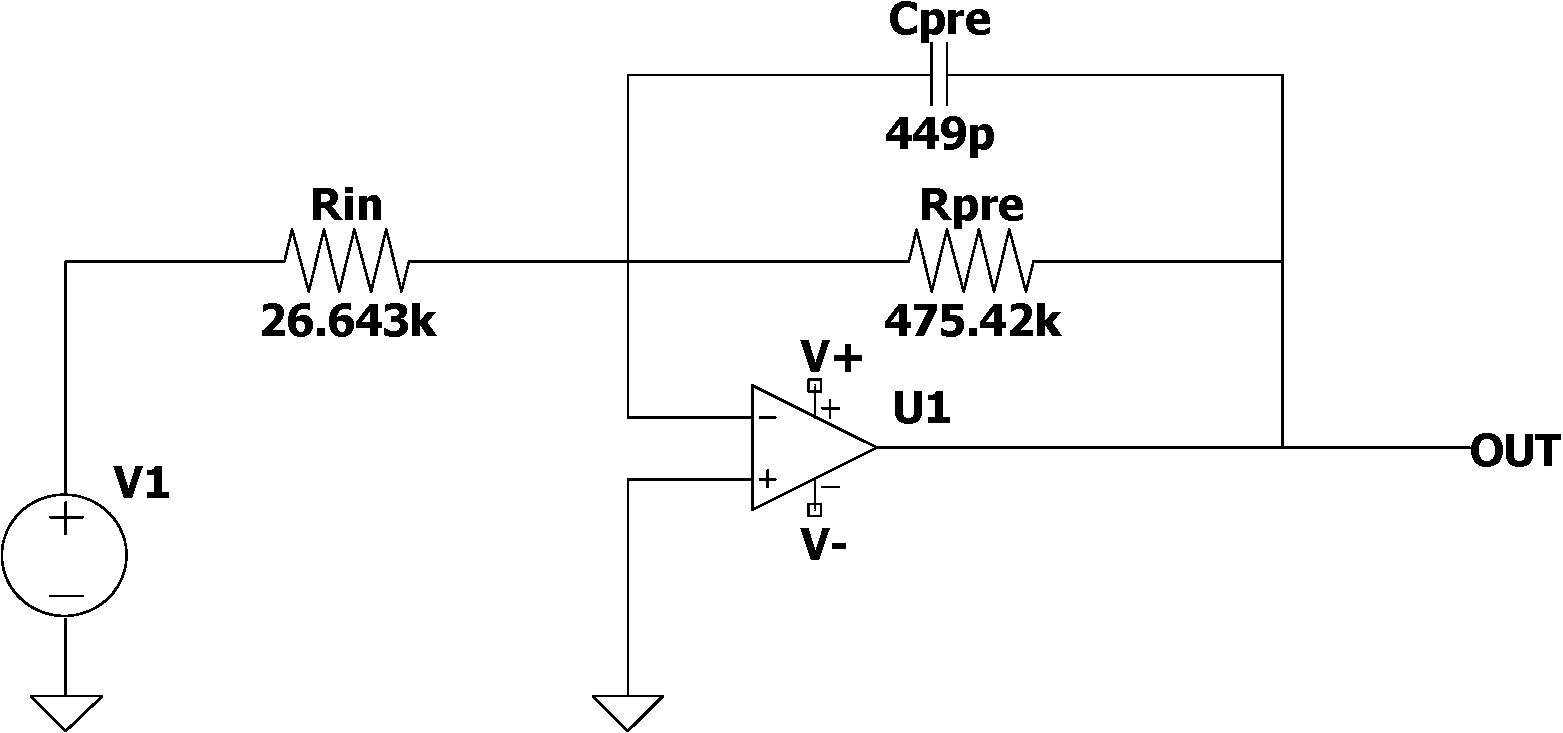
\includegraphics[scale=0.3, angle=0]{preamp.pdf}
\caption{ Circuito amplificatore di carica }
\label{fig:preamp}
\end{figure}
\end{center}

la cui funzione di trasferimento è data, nel formalismo di Laplace, da

\begin{equation}
    \label{eqn:preamp_Laplace}
    H(s) = -\frac{R_{pre}}{R_{in}} \frac{1}{1+sR_{pre}C_{pre}}
\end{equation}

in cui possiamo effettuare la sostituzione $s \longleftrightarrow i\omega$ per riprodurre la soluzione stazionaria. Considerando poi
solamente il modulo, e definendo il tempo caratteristico $\tau_{pre}=R_{pre}C_{pre}$, avremo

\begin{equation}
    \label{eqn:preamp_trasf}
    H(\omega) = \frac{R_{pre}}{R_{in}} \frac{1}{\sqrt{1+\omega^2\tau_{pre}^2}}
\end{equation}

Si osserva inoltre che inserendo nella formula \ref{eqn:preamp_Laplace} la trasformata di Laplace dell'impulso di tensione, pari a 
$V_{in}$/s, si otterrà in uscita, antitrasformando opportunamente, un segnale esponenziale corrispondente a

\begin{equation}
    \label{eqn:Vout1_preamp}
    V_{pre}^{pulse}(t) = -\frac{R_{pre}}{R_{in}}V_{in}(1-e^{-\frac{t}{\tau_{pre}}})
\end{equation}

Quest'ultima è valida finché dura l'impulso di tensione: essendo $T_{pulse} << \tau_{pre}$, potremo considerare l'espansione in 
serie di Taylor della \ref{eqn:Vout1_preamp}, ottenendo una discesa lineare. Tale discesa lineare si interromperà all'esaurirsi dell'
impulso in ingresso, lasciando posto alla formula della scarica del condensatore $C_{pre}$, caricato proprio dallo stesso impulso.
Ne risulta un grafico che ha un picco negativo $V_{pre}^{max}$ in corrispondenza di t = $T_{pulse}$, per poi risalire con la curva esponenziale
dettata da

\begin{equation}
    \label{eqn:Vout2_preamp}
    V_{pre}^{RC}(t) = V_{pre}^{max}e^{-\frac{t}{\tau_{pre}}}.
\end{equation}

\subsection{Discussione dati}

Si precisa che sono stati suggeriti dei valori per i parametri del circuito $\tau_{pre,th} = 220 \mu s$ e $C_{pre} = 450 pF$, con $R_{pre}$ calcolato di 
conseguenza. Pertanto i valori misurati con il multimetro sono

\begin{align*}
    R_{pre} = (475.4 \pm 0.2)k\Omega \quad \sigma_{\%}=0.04 \% \\    
    C_{pre} = (149 \pm 14) pF \quad \sigma_{\%}=3.1 \%    \\
    \tau_{pre,th} = (213 \pm 7)\mu s \quad \sigma_{\%}=3.1 \%     \\
\end{align*}

Si è dunqueimpostato un impulso della durata di $T_{pulse}$ = $2 \mu s$: sapendo inoltre che la carica da iniettare 
corrispondeva a $Q_{in}^{th}$ = $80 pC$ e che la resistenza di ingresso scelta misurava $R_{in}=(26.64\pm0.01) k\Omega$ ($\sigma_{\%}=0.04\%$), 
si è selezionata l'altezza $V_{in}$ dell'impulso in modo che fosse soddisfatta la relazione

\begin{equation}
    \label{eqn:Qin}
    Q_{in} = \frac{V_{in}}{R_{in}} T_{pulse}.
\end{equation}

Ne si è ricavato $V_{in}^{th}$ =1.06 V. Per controllare la correttezza del circuito si è misurato il picco $V_{pre}^{max}$, che sarà
dato, utilizzando l'approssimazione della \ref{eqn:Vout1_preamp}, da

\begin{equation}
    \label{eqn:Vpre_max}
    V_{pre}^{max} = -\frac{R_{pre}}{R_{in}} V_{in} \frac{T_{pulse}}{\tau_{pre}} = - \frac{Q_{in}}{C_{pre}}
\end{equation}

da cui, inserendo il valore misurato $V_{in}^{th}=(1.02\pm 0.02) V$, si ricava $V_{pre,th}^{max} =  (-170 \pm 6) mV$. Invece dalla 
misura si ottiene $V_{pre,sper}^{max} = (-176 \pm 4) mV$, per cui $\lambda = 0.76$ e lo scostamento percentuale è $\epsilon = 3.2 \%$, 
ossia il valore misurato è ottimamente compatibile con quello atteso.

Si è inoltre la verificata la linearità tra $Q_{in}$ e $V_{pre}^{max}$ descritta da \ref{eqn:Vpre_max} variando la durata dell'impulso
in ingresso e quindi la carica iniettata nel circuito secondo \ref{eqn:Qin}. Si riportano quindi in grafico i punti, la retta 
interpolante e i principali parametri di bontà del fit. 

\begin{center}
\begin{figure}[H]
\centering
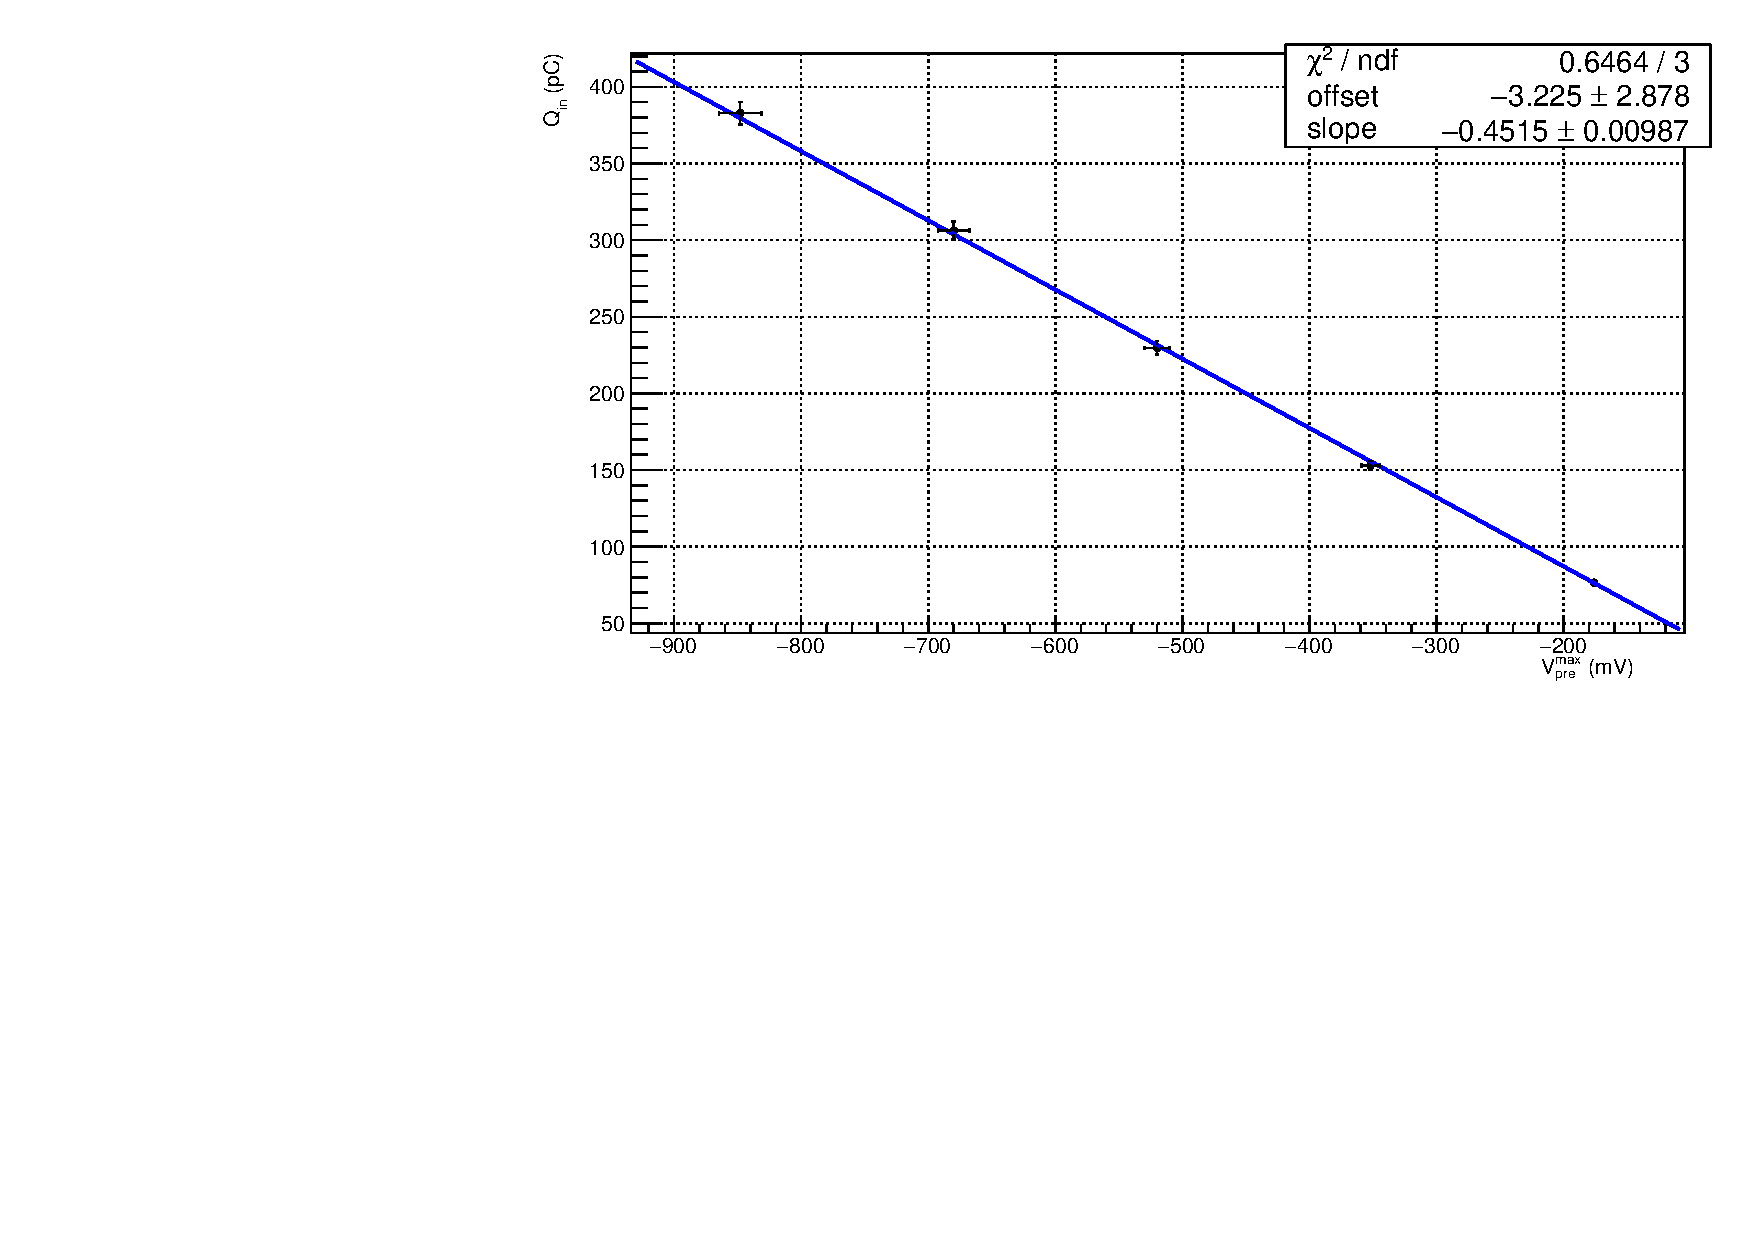
\includegraphics[scale=0.4, angle=0]{fitpreamp.pdf}
\caption{Carica iniettata e picco di tensione in uscita}
\label{fig:QinvsVpre}
\end{figure}
\end{center}

\begin{center}
\begin{figure}[H]
\centering
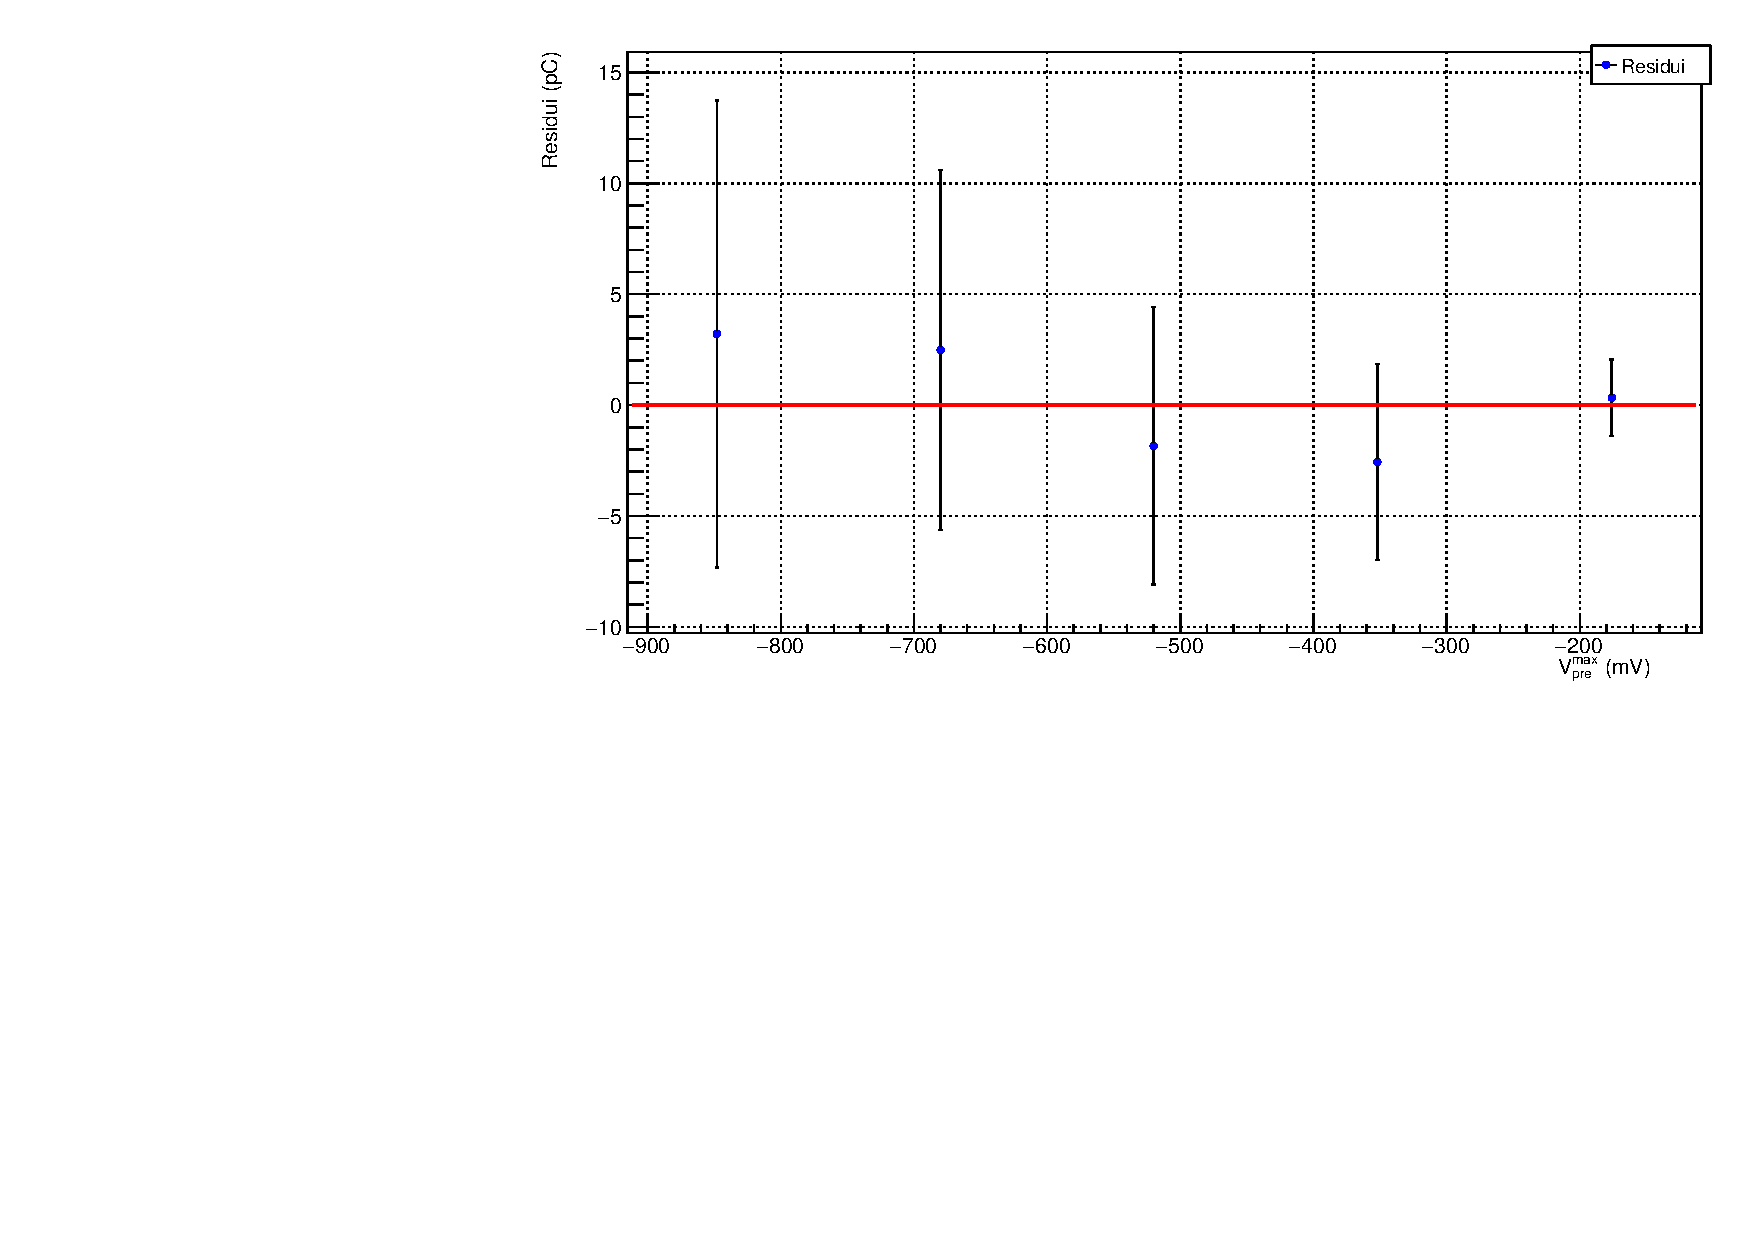
\includegraphics[scale=0.4, angle=0]{residuipreamp.pdf}
\caption{Grafico dei residui della relazione tra $Q_{in}$ e $V_{pre}^{max}$}
\label{fig:QinvsVpre_res}
\end{figure}
\end{center}

\begin{table}[ht]
    \centering
    \begin{tabular}{ccccc}
        \toprule
        $\sigma_{y, post}$    &$\chi^{(2)}$    &$\lambda_{\chi}$   &$\rho$ &t      \\
        \midrule
        3.0 pC                  &0.65            &0.96               &-0.9998&-109.14\\
        \bottomrule
    \end{tabular}
    \caption{parametri di verifica della bontà del fit}
\end{table}

Gli estimatori danno tutti risposta positiva, quindi possiamo concludere che la relaizone lineare è ben verificata.
Inoltre dal valore di pendenza, considerando la legge lineare \ref{eqn:Vpre_max}, è possibile ottenere una stima sperimentale della capacità $C_{pre}$, 
da confrontare con il valore misurato. Si ricava quindi $C_{pre,sper} = (452\pm 10)pF$, che ha $\lambda = 0.15 $ rispetto al valore misurato.

Inoltre dallo studio della \ref{eqn:Vout2_preamp}, e in particolare della sua linearizzazione logaritmica, è possibile ricavare
una stima sperimentale di $\tau_{pre}$. Infatti applicando il logaritmo naturale ottengo

\begin{equation}
    \log V(t) = \log V_{pre}^{max} - \frac{t}{\tau_{pre}}
\end{equation}

per cui si trova una relazione lineare tra $\log V(t)$ e t, da cui $\tau_{pre}$=-1/b con b slope del fit.
Si riporta il grafico di tempi e lograitmi delle tensioni, interpolati linearmente, e il relativo grafico dei residui

\begin{center}
\begin{figure}[H]
\centering
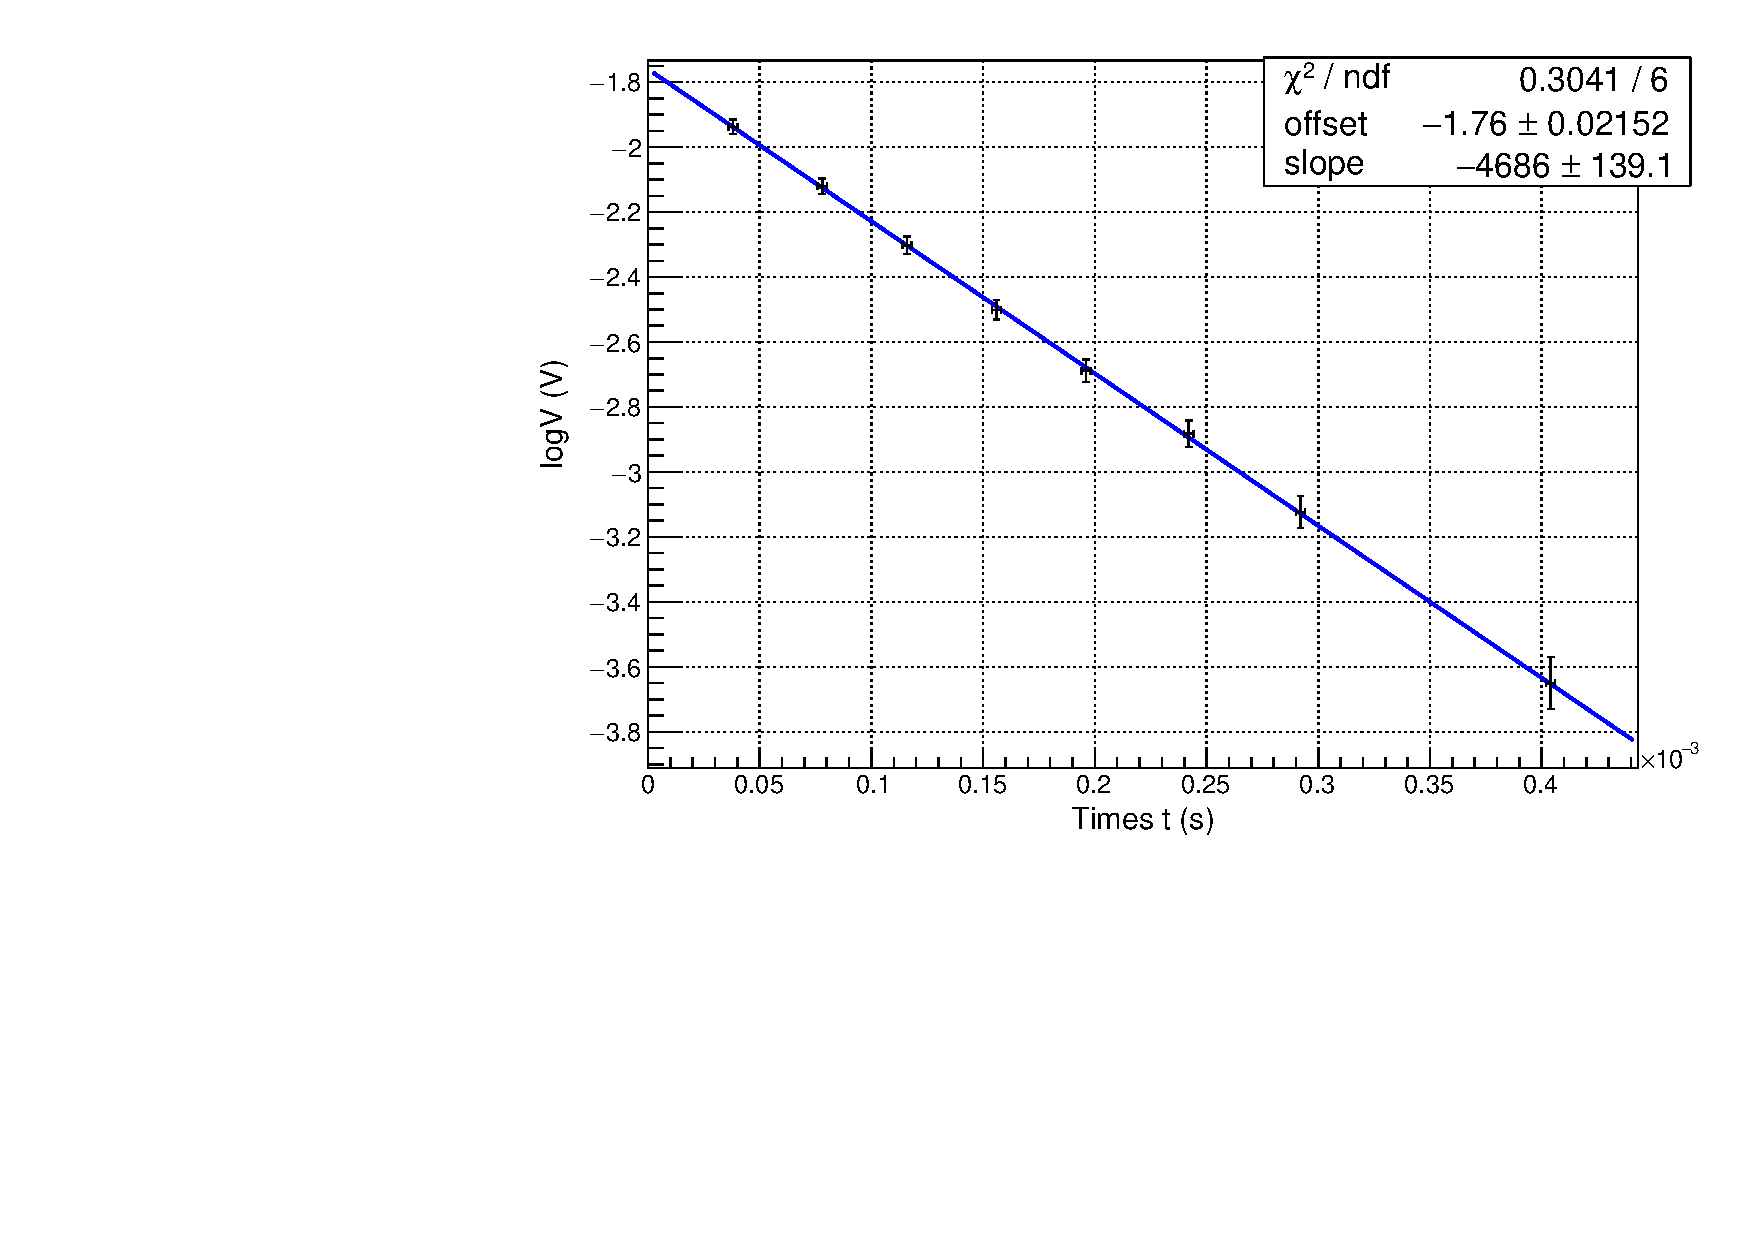
\includegraphics[scale=0.4, angle=0]{preampRC.pdf}
\caption{Relazione lineare tra logaritmi delle tensioni e tempi}
\label{fig:QinvsVpre}
\end{figure}
\end{center}

\begin{center}
\begin{figure}[H]
\centering
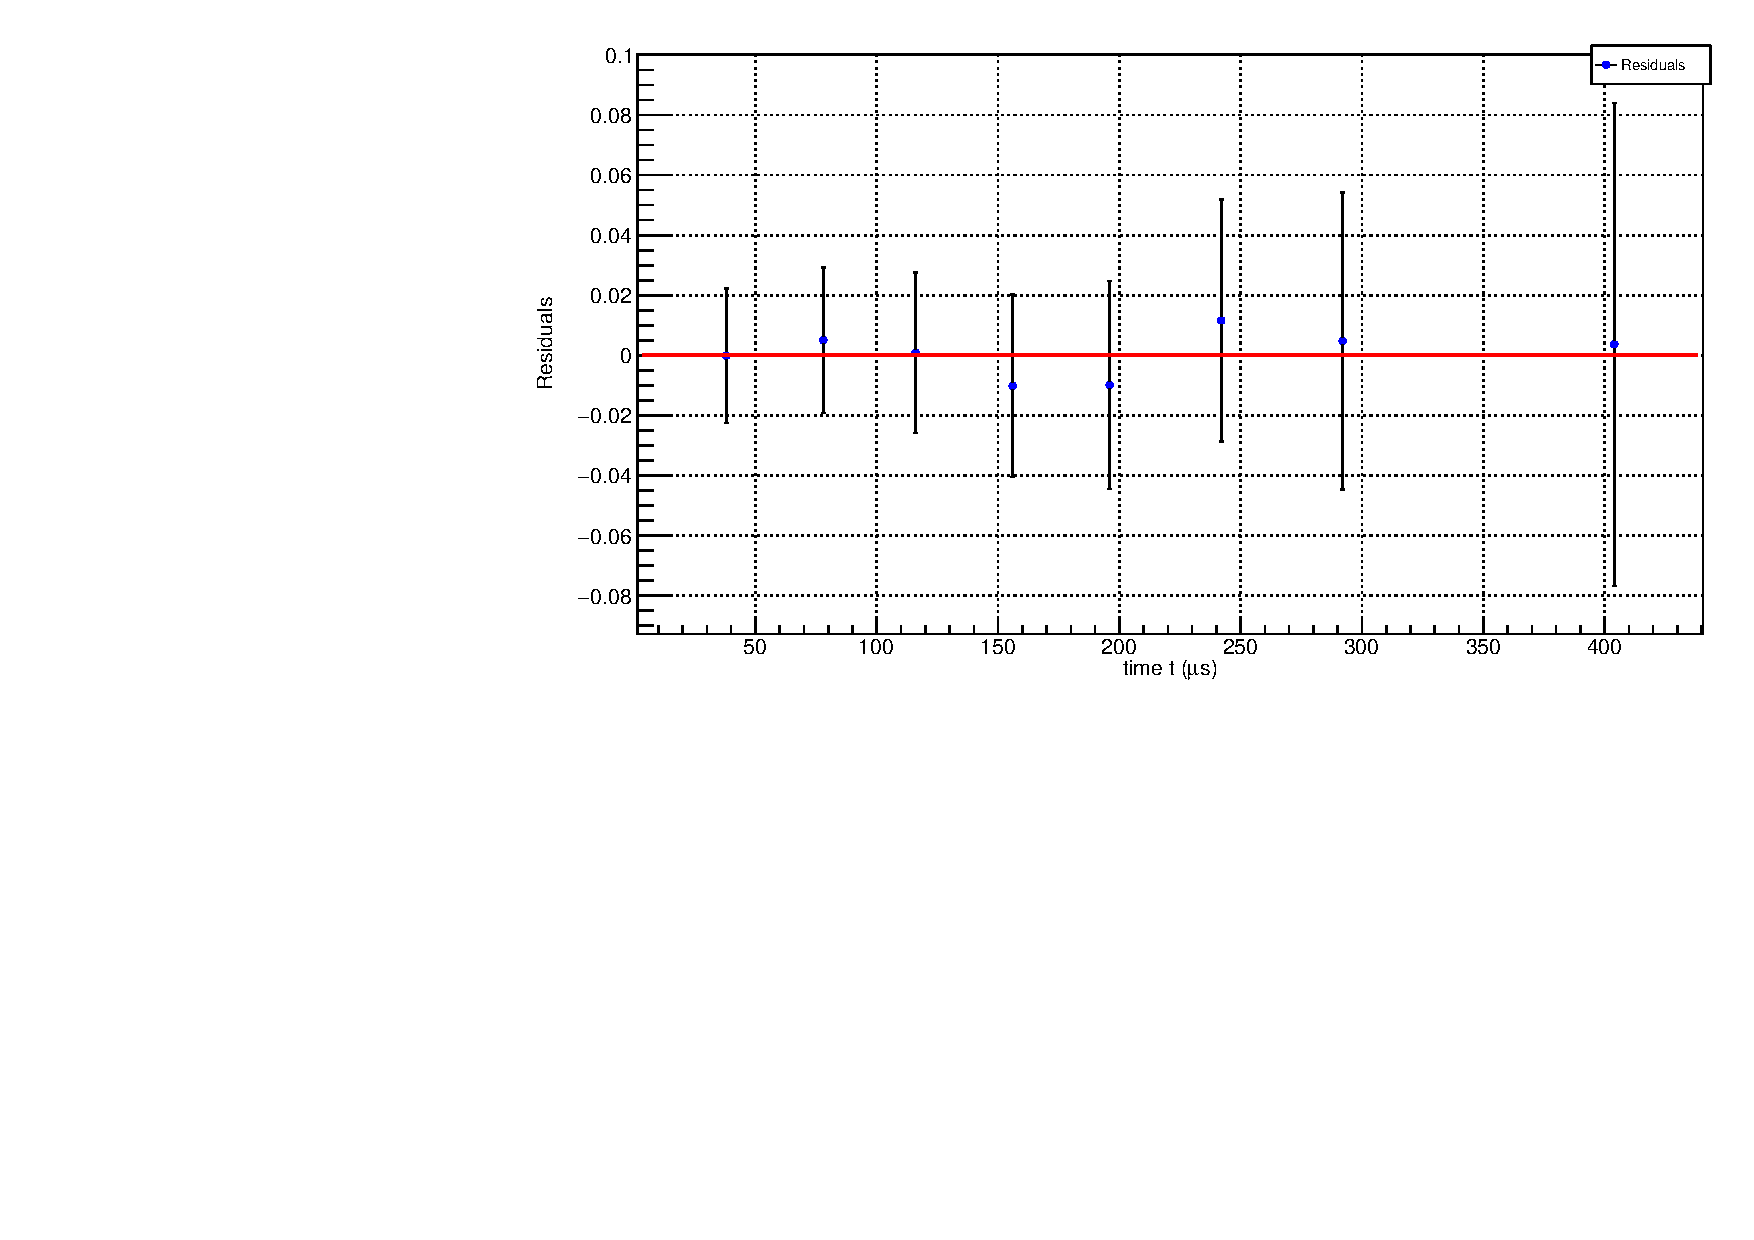
\includegraphics[scale=0.4, angle=0]{preampRCresidui.pdf}
\caption{Grafico dei residui della relazione tra $\log V$ e t}
\label{fig:QinvsVpre}
\end{figure}
\end{center}

\begin{table}[ht]
    \centering
    \begin{tabular}{ccccc}
        \toprule
        $\sigma_{y, post}$    &$\chi^{(2)}$    &$\lambda_{\chi}$   &$\rho$  &t   \\
        \midrule
        0.008 V               &0.33            &1.64              &-0.99991&-189.59\\
        \bottomrule
    \end{tabular}
    \caption{parametri di verifica della bontà del fit}
\end{table}

Dal valore della pendenza, come anticipato prima, ricaviamo una stima di $\tau_{pre,sper}$. A scopo di controllo, è inoltre possibile 
ottenere una valutazione di $V_{pre}^{max}$ usando il parametro di offset a sapendo $V_{pre}^{max} = e^a$. Si riportano quindi i due
valori calcolati con i loro errori calcolati per propagazione.

\[
\tau_{pre,sper} = (213 \pm 6)\mu s \quad \sigma_{\%} = 2.9 \%    
\]
\[
V_{pre}^{max} = (-172 \pm 3)mV \quad \sigma_{\%} = 2.0 \%    
\]

che risultano ottimamente compatibili con i valori attesi $V:{pre.th}^{max}$ e $\tau_{pre,th}$, in quanto $\lambda_{\tau} = 0.01$
e $\lambda_{V}=0.2$.

Si è infine effettuato uno studio in frequenza del circuito con lo scopo di verificare la \ref{eqn:preamp_trasf}, variando la frequenza
e verificando il variare del modulo dell'ampiezza di fronte a un ingresso sinusoidale.
Si riporta in particolare il grafico di Bode che raffigura frequenza e amplificazione in dB: ai punti sperimentali si è affiancata
anche la simulazione effettuata su LTspice e il modello teorico rappresentato dalla \ref{eqn:preamp_trasf}.

\begin{center}
\begin{figure}[H]
\centering
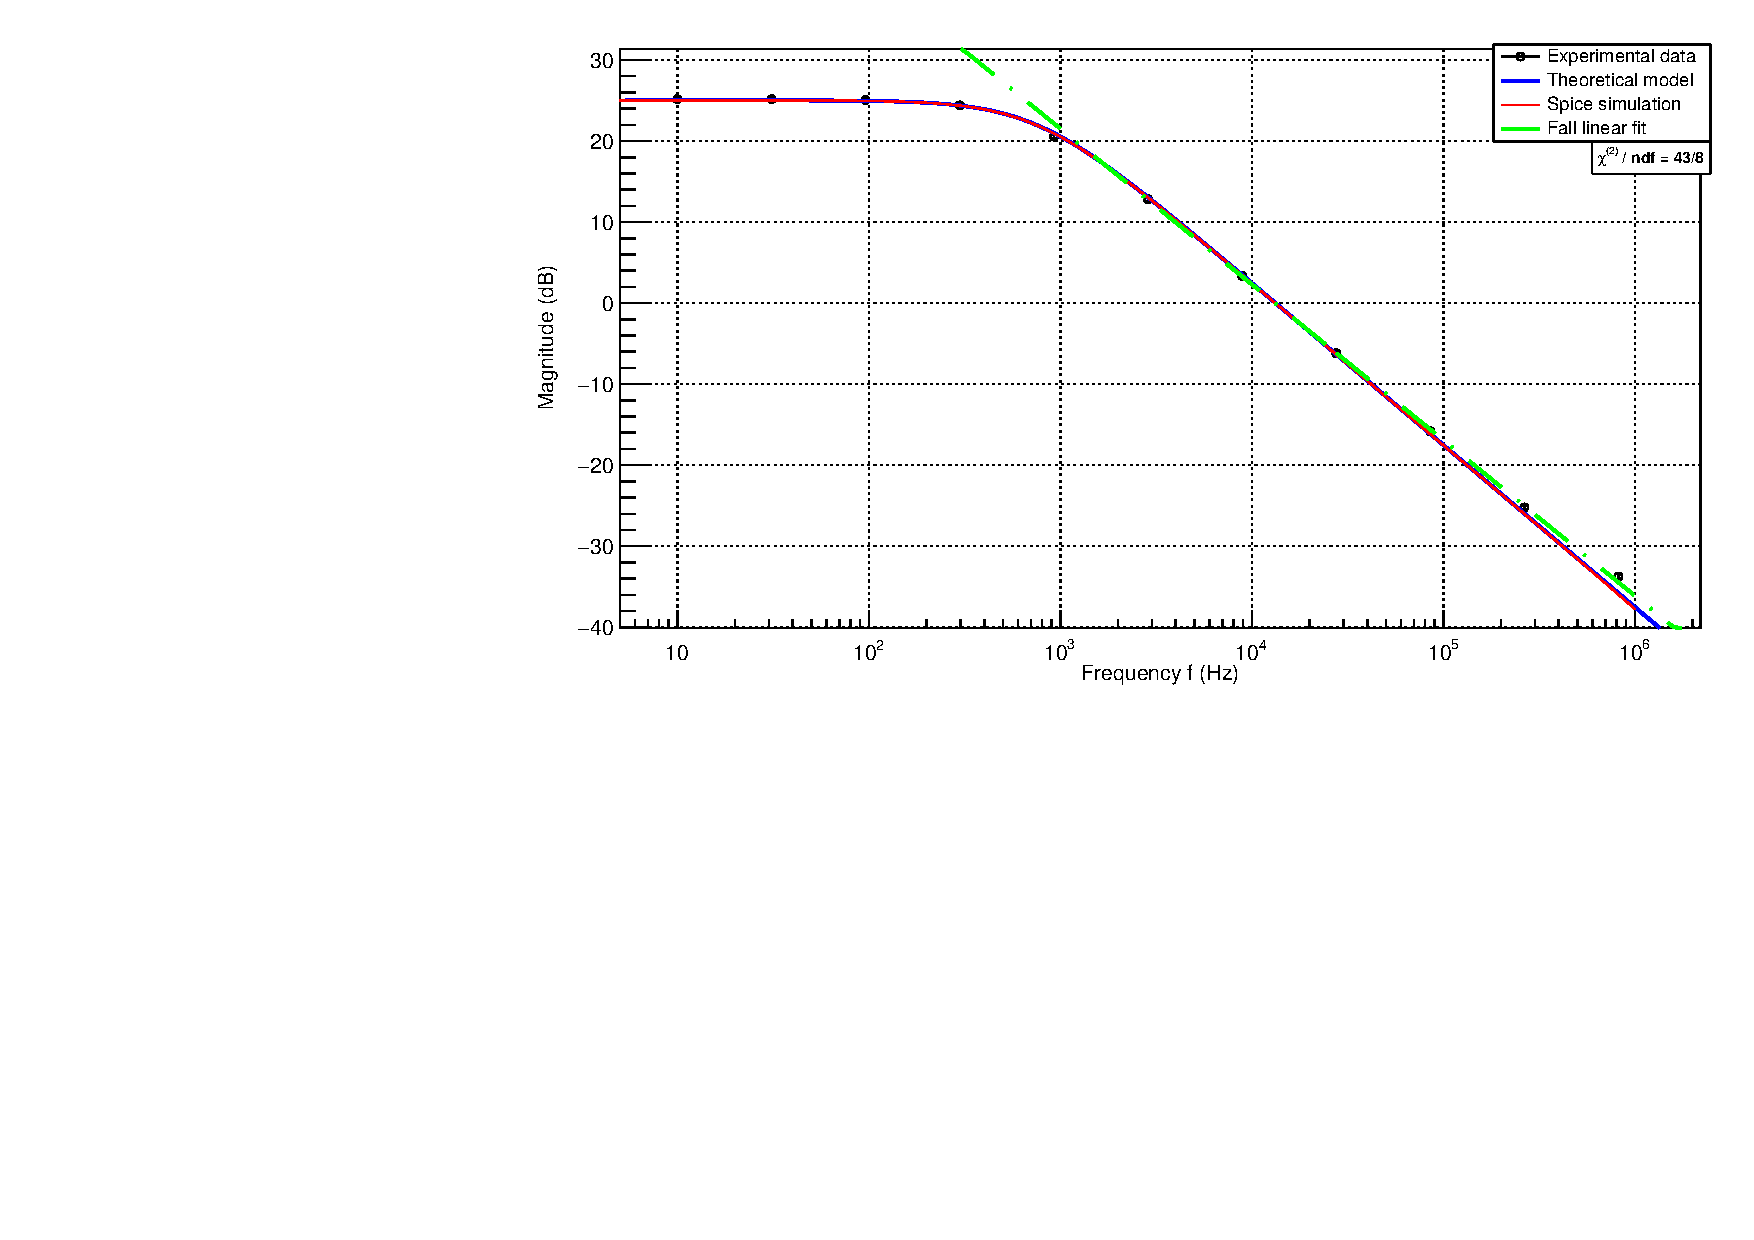
\includegraphics[scale=0.4, angle=0]{bodepreamp.pdf}
\caption{Grafico di Bode del circuito preamplificatore}
\label{fig:bodepreamp}
\end{figure}
\end{center}

Si osserva che i dati giacciono correttamente sulla simulazione e anche il modello teorico appare adeguato, nonostante il grafico 
dei residui mostri una certa incompatibilità delle alte frequenze. COMMENTO

\begin{center}
    \begin{figure}[H]
    \centering
    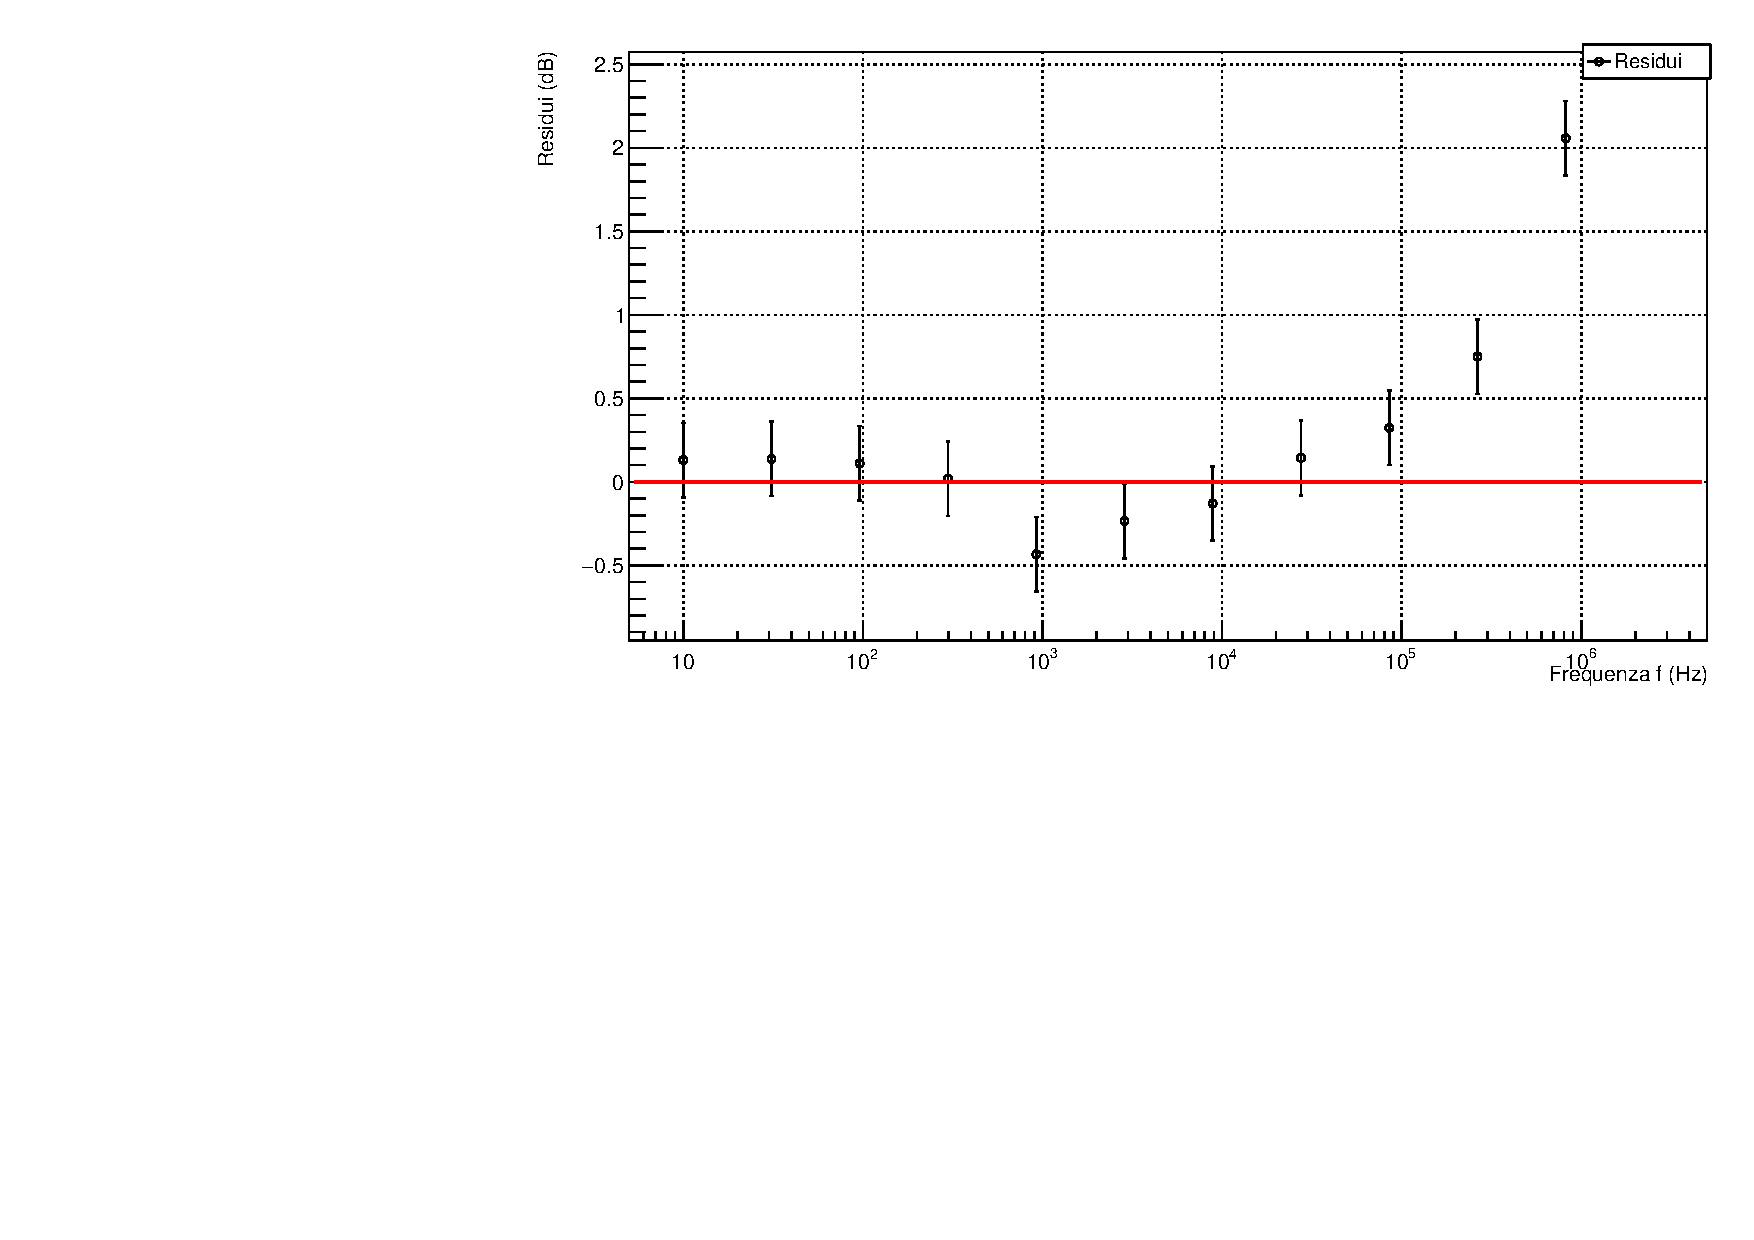
\includegraphics[scale=0.4, angle=0]{bodepreampresidui.pdf}
    \caption{Grafico del grafico di Bode}
    \label{fig:bodepreamp_res}
    \end{figure}
\end{center}

\section{Circuito formatore}
\subsection{Shaper base CR-RC}
\subsubsection{Breve discussione del circuito}

Il secondo passo per la costruzione della catena elettronica consiste invece nella costruzione del circuito formatore il cui schema è 
riportato in figura (\ref{fig:shaper}), che dia per l'appunto una forma al segnale, tipicamente simile a un profilo gaussiano.

\begin{center}
    \begin{figure}[H]
    \centering
    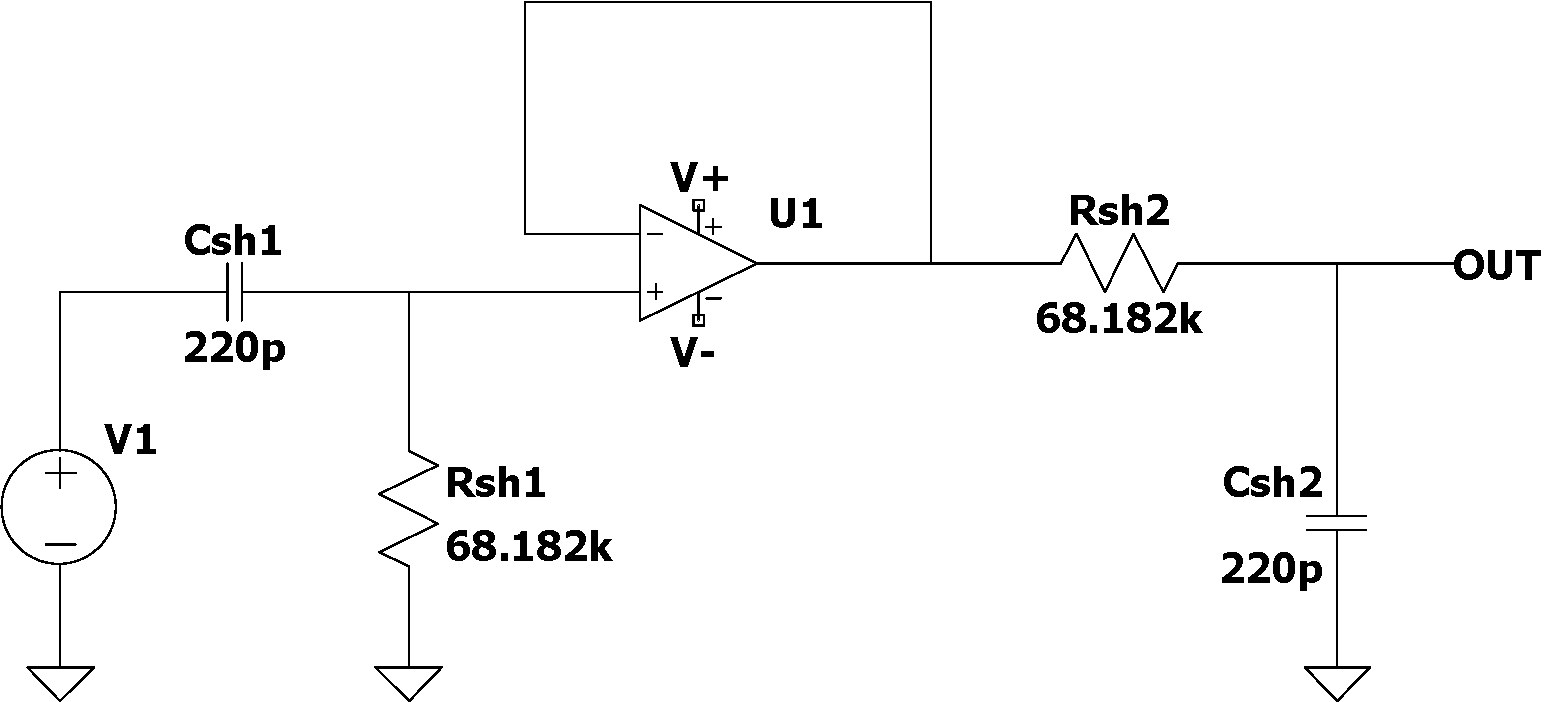
\includegraphics[scale=0.3, angle=0]{shaper.pdf}
    \caption{Circuito formatore}
    \label{fig:shaper}
    \end{figure}
\end{center}
    
Si osserva che il circuito è costruito tramite due stadi RC e CR, disaccoppiati tramite un buffer costruito utilizzando il secondo 
opamp presente nel TL082.

Si specifica inoltre che i valori di $C_{sh}^{(1)}=C_{sh}^{(2)}$ e $R_{sh}^{(1)}=R_{sh}^{(2)}$ sono stati scelti in modo da ottenere 
il valore di $\tau_{sh}$ indicato nel logbook.

Trattando il circuito con Laplace e considerando la fase stazionaria, si ottiene che la funzione di trasferimento in funzione di 
$\omega$ è la seguente:
\begin{equation}
H(\omega)=\frac{\omega \tau}{1+\omega^2\tau^2}
\end{equation}

In particolare, inserendo in ingresso un'onda quadra tra 0 e $V_0$ si ottiene la funzione $V_{out}(t)$ facendo l'antitrasformata 
dal dominio delle frequenze:

\begin{equation}
    \label{eqn:V_sh}
    V_{out}(t)= - \frac{V_0}{\tau} t \cdot e^{-\frac{t}{\tau}}
\end{equation}
    

\subsubsection{Discussione dei dati}
Si è nuovamente impostata sul generatore di funzioni un'onda quadra di frequenza di 100 Hz e ampiezza pari a $V_{in}^{th}=(992 \pm 15)mV$
in modo che simuli il comportamento di un preamplificatore ideale che mantenga il segnale alto per un tempo indefinito.

Sapendo che $\tau_{th}=R_{sh}^{(1)} C_{sh}^{(1)} = R_{sh}^{(2)} C_{sh}^{(2)}=22 \mu s$ si sono scelti e misurati i seguenti valori:

\begin{align*}
R_{sh}^{(1)} = (68.31  \pm 0.03)k\Omega \quad\quad \sigma_{\%}=  0.04 \% \\
R_{sh}^{(2)} = (68.075  \pm 0.03)k\Omega \quad\quad \sigma_{\%}=  0.04\% \\
C_{sh}^{(1)}= (234 \pm  9)pF \quad\quad \sigma_{\%}= 4 \% \\
C_{sh}^{(2)}= (234 \pm  9)pF \quad\quad \sigma_{\%}= 4 \% \\
\end{align*}

dove l'errore è stato calcolato secondo quanto scritto in appendice tenendo conto delle specifiche del multimetro Metrix 32292 relative
ad un fondoscala di 100 k$\Omega$ per le resistenze e di 1000 pF per le misure delle capacità.

Mediante i cursori si è quindi misurato il valore massimo (in valore assoluto) $V_{sh}^{max}=(346 \pm 6)mV$ e il tempo corrispondente 
$\tau_{sh}^{max}=(16 \pm 1)\mu s$.

Si è poi verificata la correttezza del trasferimento immettendo nel circuito un'onda quadra di altezza 1V e misurando un set di 10 punti 
della curva in uscita, indicata dal modello in \ref{eqn:V_sh}. In particolare però per l'identificazione della curva teorica si è 
scelto di non utilizzare il $\tau_{sh,sper}$ ma bensì di sfruttarlo come parametro per applicare il metodo del minimo $chi^{(2)}$, 
ossia vagliare i valori del $\chi_{(2)}$ rispetto ai dati sperimentali al variare di $\tau_{sh}$ e quindi
della curva teorica e poi scegliere il tempo caratteristico per cui l'estimatore risulta avere un minimo. 
La scelta del minimo è stata effettuata tramite un fit parabolico in prossimità della convessità, e calcolando l'ascissa del 
vertice della parabola.
L'errore di $\tau_{sh}$ è dato dalla semidispersione ottenuta facendo riferimento all'intervallo [$\tau_+ ; \tau_-$] 
tali per cui $\chi^{(2)}_{\pm} = \chi^{(2)}_{min} + 1$.

\begin{center}
    \begin{figure}[H]
    \centering
    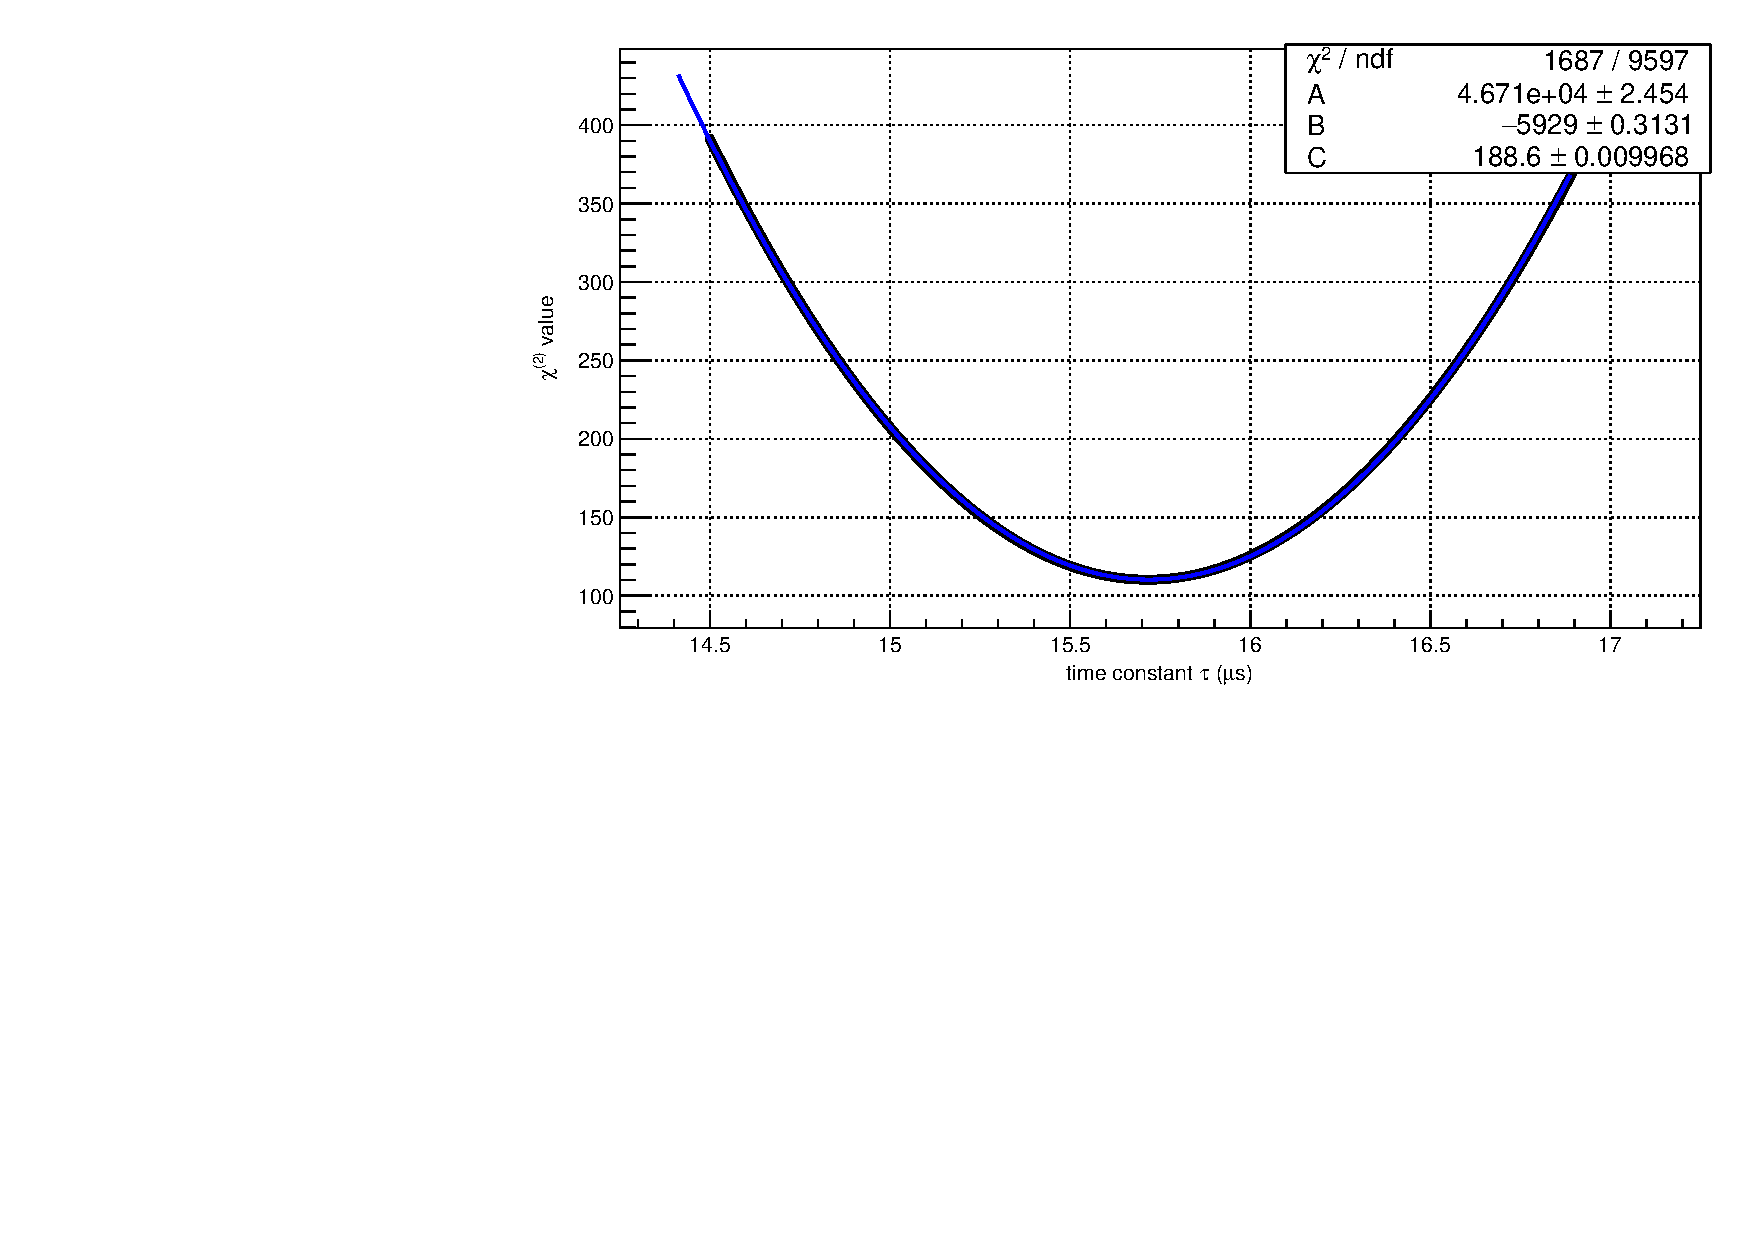
\includegraphics[scale=0.375, angle=0]{chi_forma_no_pz.pdf}
    \caption{Andamento di $chi_{(2)}$ al variare di $\tau_{sh}$}
    \label{fig:chi_forma_no_pz}
    \end{figure}
\end{center}

Da cui si sceglie $\tau_{sh} = (\pm) \mu s$. Da tale decisione si può plottare il modello teorico assieme ai dati come fatto nel
grafico seguente

\begin{center}
    \begin{figure}[H]
    \centering
    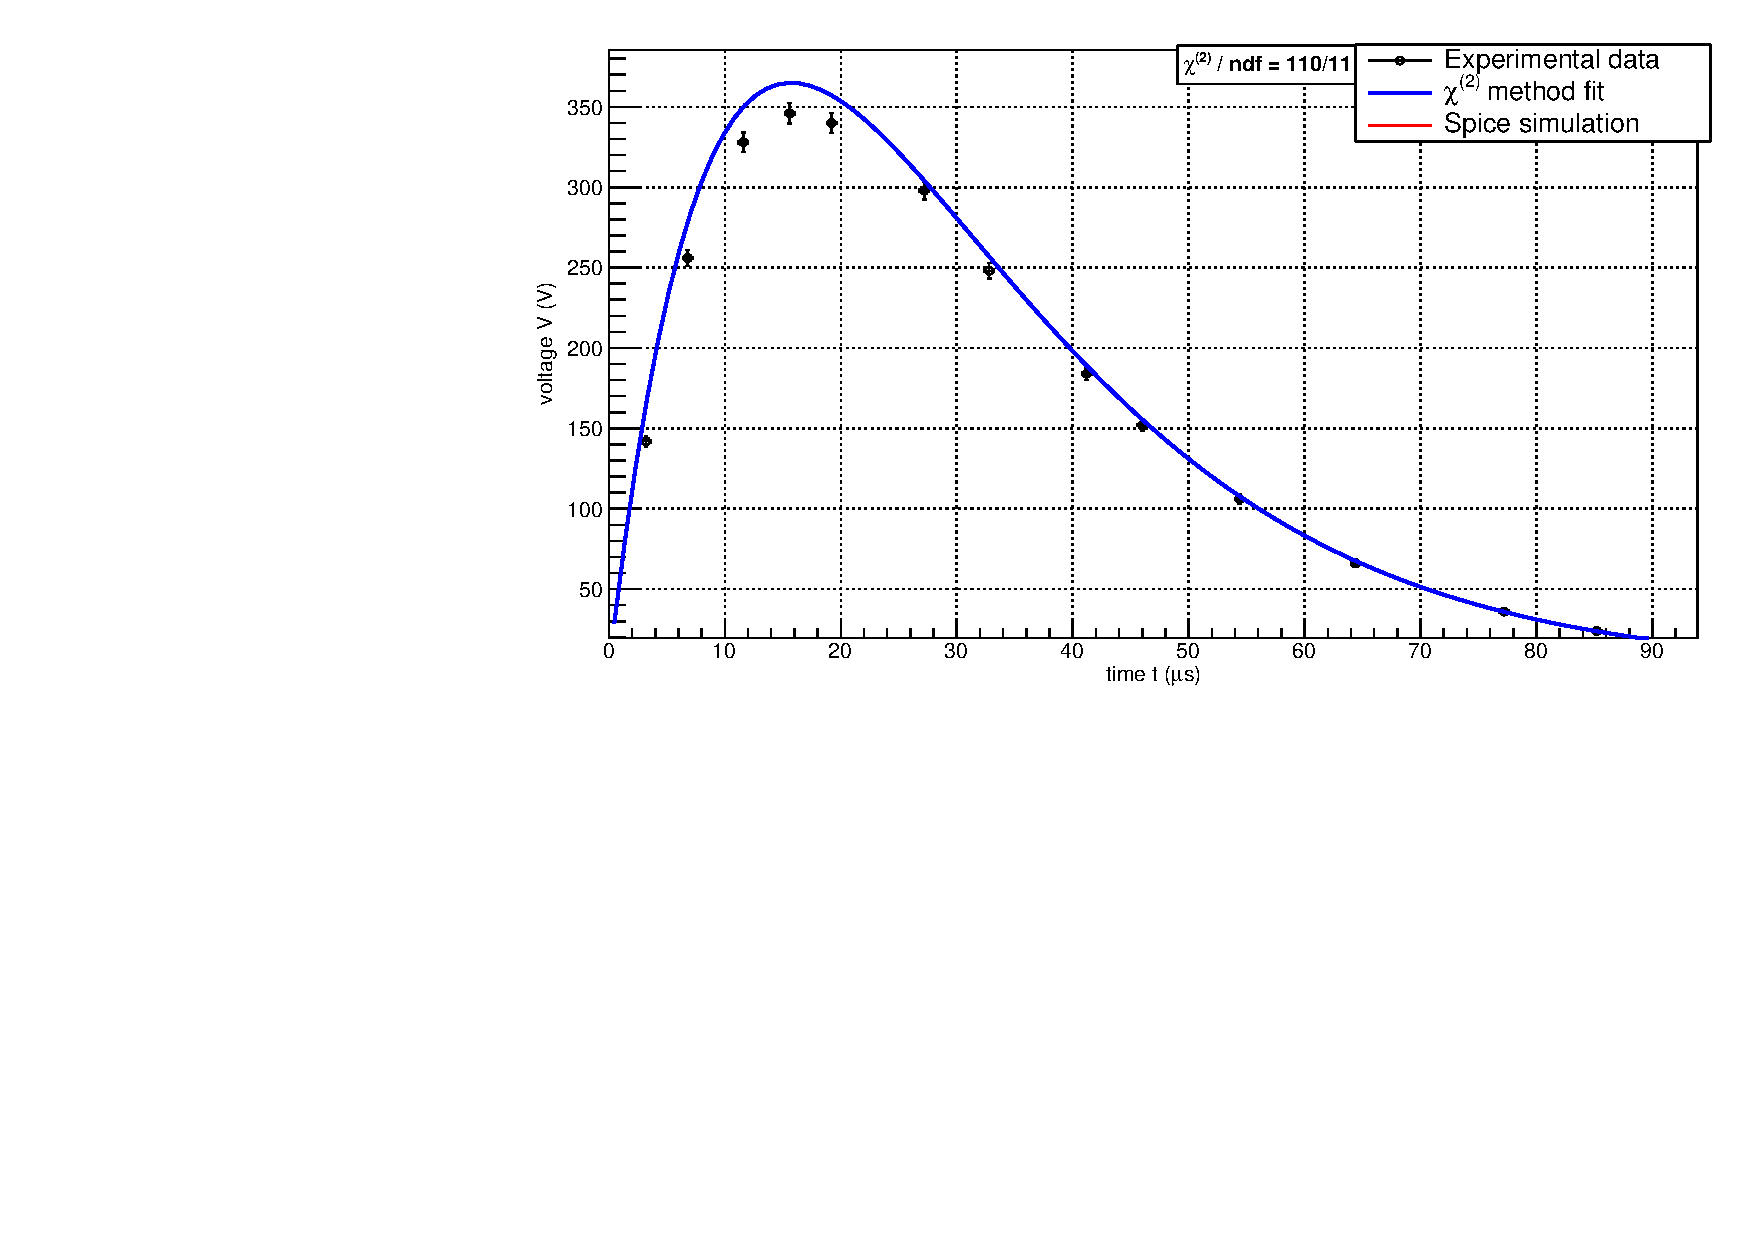
\includegraphics[scale=0.375, angle=0]{forma_no_pz.pdf}
    \caption{Risposta del circuito formatore a un'onda quadrata in ingresso}
    \label{fig:forma_no_pz}
    \end{figure}
\end{center}

Si vede che i dati non sono compatibili con il modello teorico, in quanto pur riproducendone l'andamento risultano sensibilmente 
staccati. Questo è dovuto a mi scusi ma io che cazzo ne so

Si è infine nuovamente studiato il comportamento del circuito al variare della frequenza (le misure sono riportate in appendice); si è 
ottenuto il seguente grafico di Bode (fig (\ref{fig:bodeshaper_no_pz})); al fine di ottenere un confronto immediato sono plottate 
sovrapposte la curva teorica relativa ai dati sperimentali ed il fit dei dati ottenuti mediante la simulazione di LT-spice:

\begin{center}
    \begin{figure}[H]
    \centering
    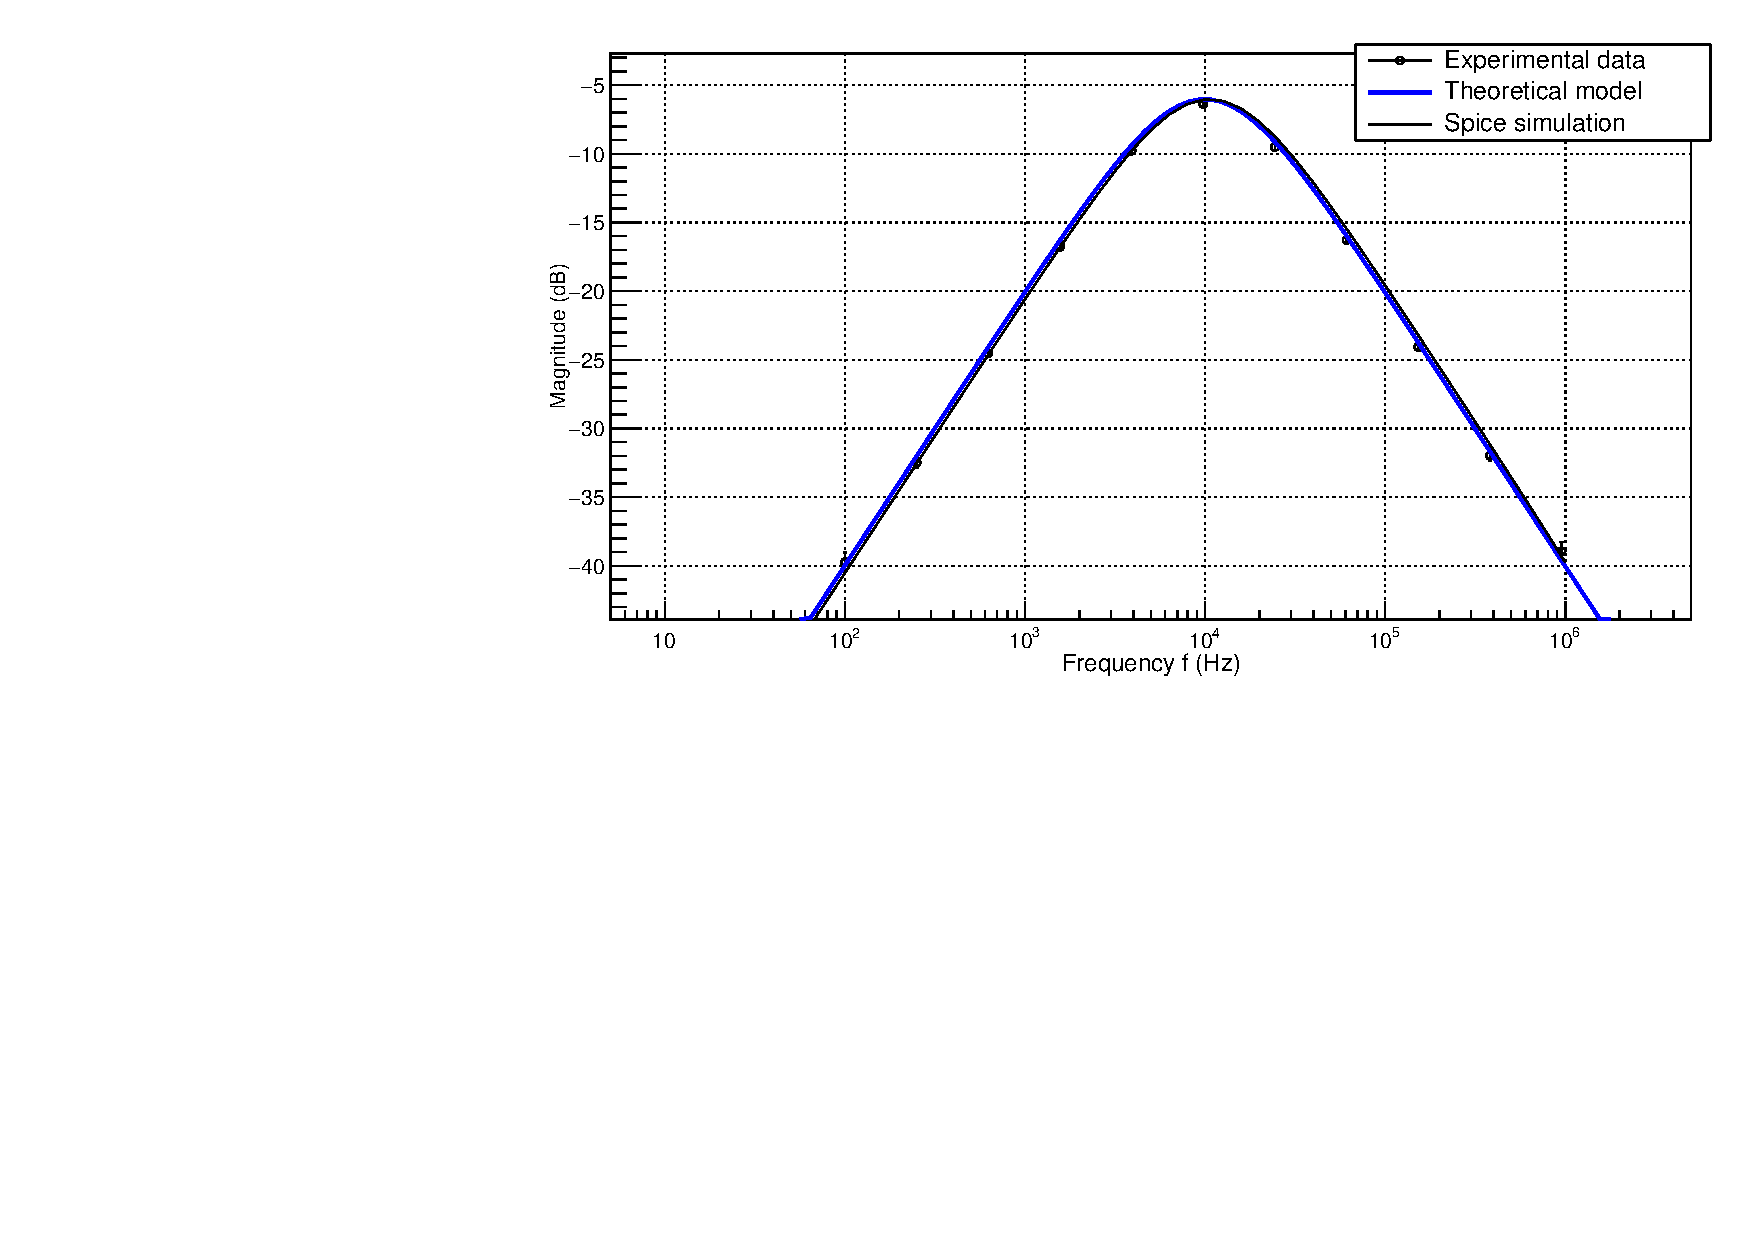
\includegraphics[scale=0.375, angle=0]{bodeshaper_no_pz.pdf}
    \caption{Grafico di Bode}
    \label{fig:bodeshaper_no_pz}
    \end{figure}
\end{center}

Si osserva il diverso comportamento dello shaper base, che opera come derivatore per frequenze basse e come integratore a frequenze
alte.

Si riporta quindi l'andamento dei residui:
\begin{center}
    \begin{figure}[H]
    \centering
    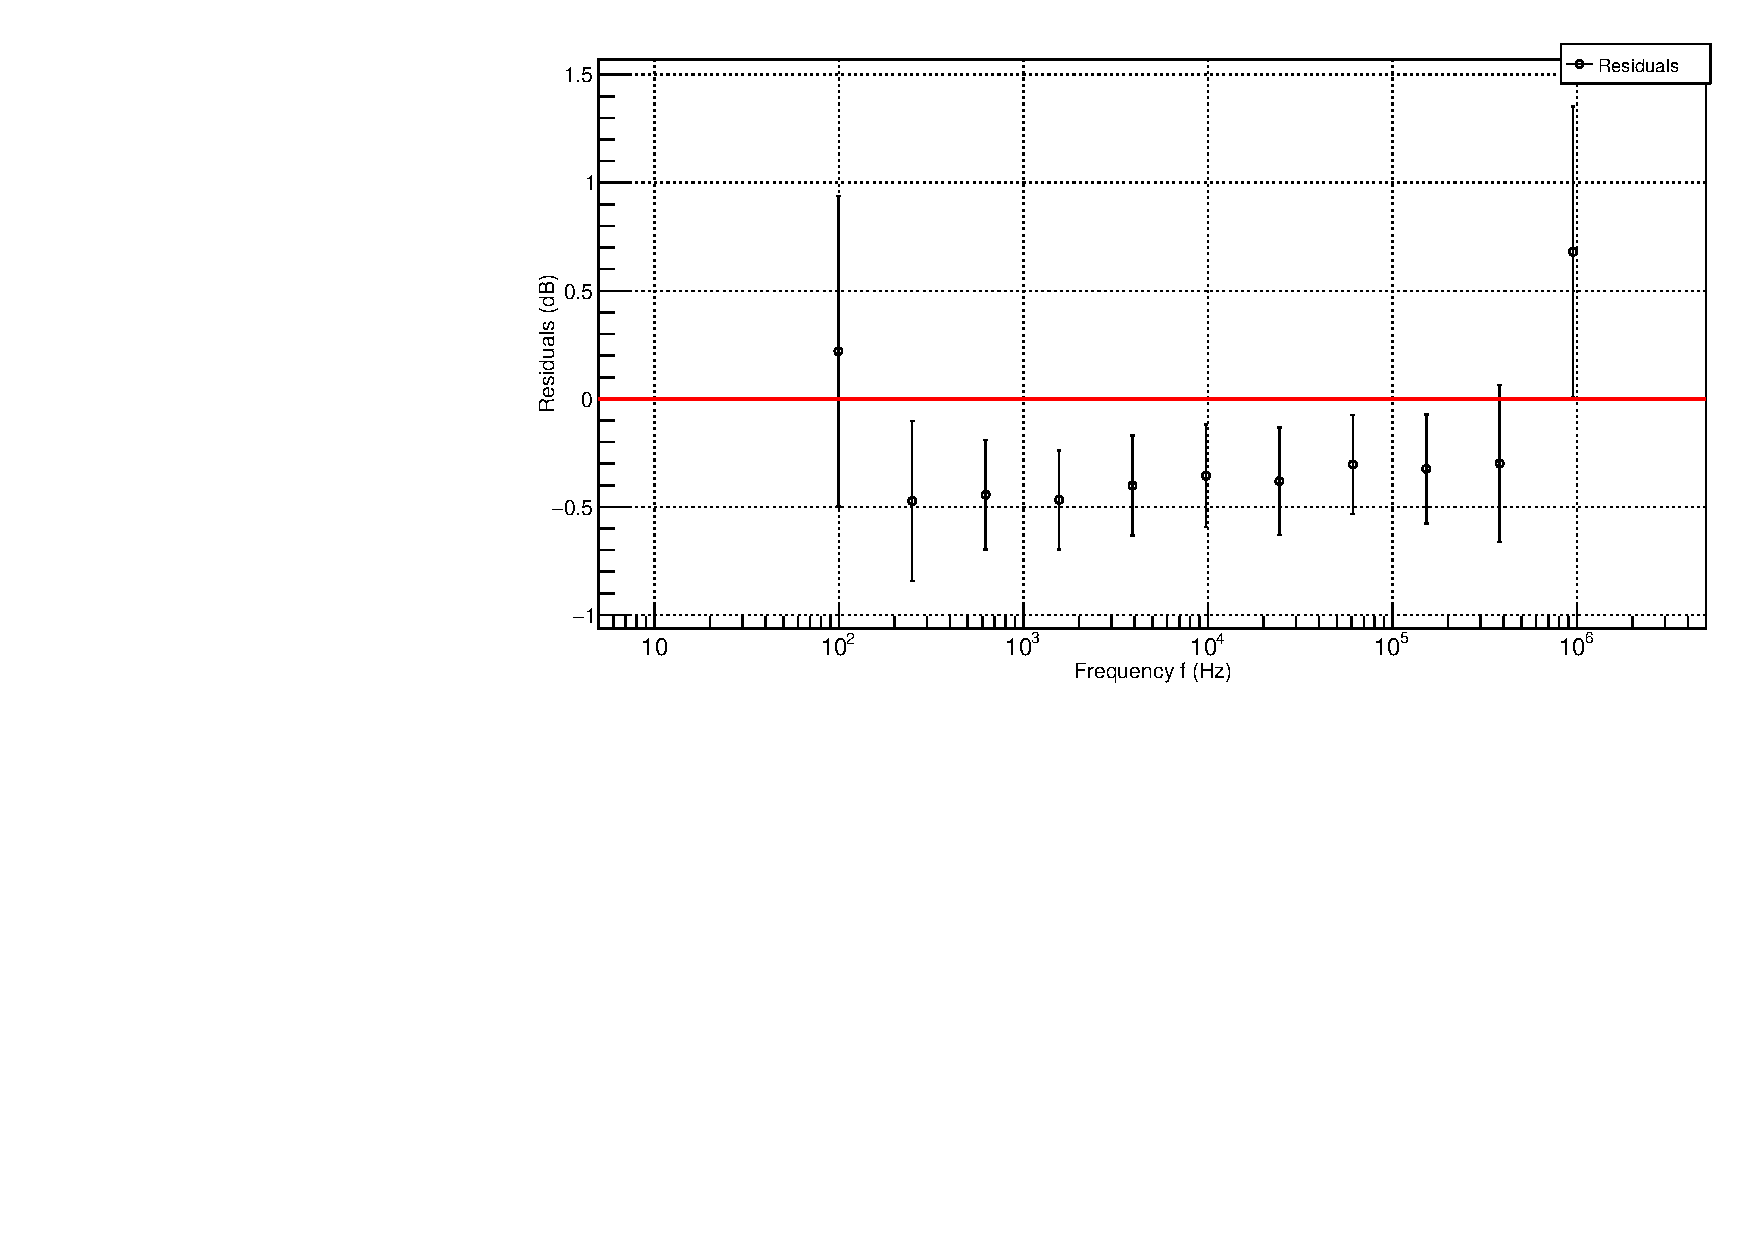
\includegraphics[scale=0.3875, angle=0]{bodeshaperresidui_no_pz.pdf}
    \caption{ Grafico dei residui (Bode)}
    \label{fig:bodeshaperresidui_no_pz}
    \end{figure}
\end{center}

\subsection{Shaper compensato}
\subsubsection{Breve discussione del circuito}
Si è proceduto inserendo come segnale in ingresso dello shaper il segnale di uscita del preamplificatore. Subentra quindi il problema 
di dover compensare l'effetto del pole-zero: infatti, se si considera in ingresso un segnale del tipo 
$V_{in}(t)=V_0 e^{-\frac{t}{\tau_{pre}}}$ si ottiene la seguente trasformata di Laplace :

\begin{equation}
    V_{in}(s)=\frac{Vo}{s+\frac{1}{\tau_{pre}}}    
\end{equation}

che presenta un polo in $-\frac{1}{\tau_{pre}} $,  responsabile dell’undeshoot del segnale.
Il segnale in uscita dal primo stadio (CR) del formatore sarà quindi: $V_{out}(s)^{CR}=\frac{V_{0}}{s+\frac{1}{\tau_{sh}}}$;
si osserva quindi che inserendo una resistenza $R_{pz}$ in parallelo a $C_{sh}^{(1)}$ si ottiene invece:

\begin{equation}
    V_{out}(s)^{CR}=\frac{V_{0}}{s+\frac{1}{\tau_{sh}}}\cdot \frac{s+\frac{1}{\tau_{pz}}}{s+\frac{1}{\tau_{\parallel}}}    
\end{equation}

l’effetto del polo del preamplificatore è quindi annullato con quello dello zero del CR compensato.

Inoltre se $R_{sh}^{(1,2)}$ << $R_{pz}$ si ha $\tau_{\parallel} \approx \tau_{sh}$ e la situazione risulta quindi completamente 
analoga a quella precedente in cui si aveva un segnale in ingreso a gradino.

Lo schema del circuito dello shaper compensato è quindi il seguente:
 
\begin{center}
    \begin{figure}[H]
    \centering
    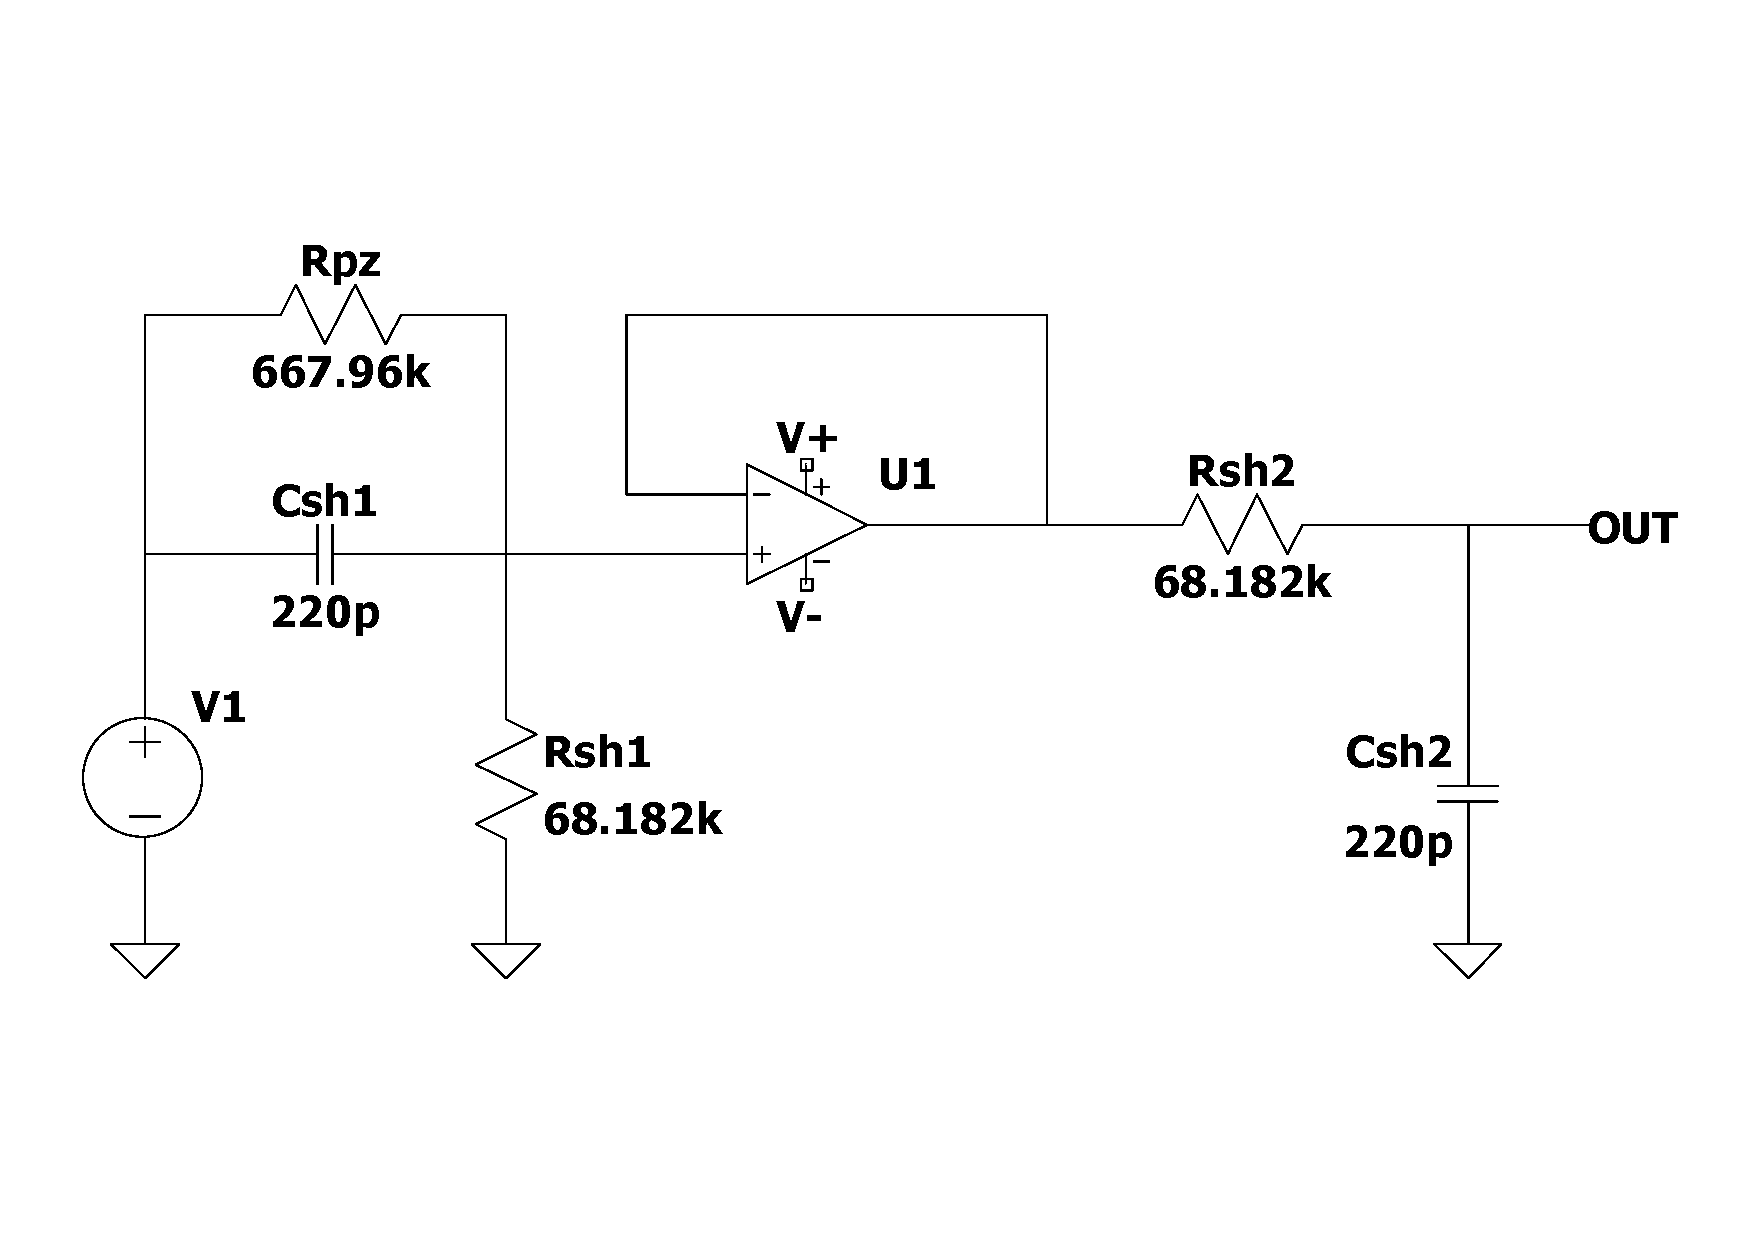
\includegraphics[scale=0.3, angle=0]{shapercomp.pdf}
    \caption{Circuito formatore con compensazione}
    \label{fig:shaper}
    \end{figure}
\end{center}
dove $V_1$ è il segnale in uscita dal preamplificatore.

%\begin{multline}
%H(\omega)=\frac{1}{(1+(\omega\tau)^2)}\cdot \frac{R_{sh} }{}

%\end{multline}

\subsubsection{Discussione dei dati}

Si è osservato che senza utilizzando lo shaper base per un segnale esponenziale come quello fornito dal preamplificatore si ottiene il 
fenomeno dell'undershoot: infatti unendo preamp e shaper si è misurato $V_{sh, undershoot}=(346 \pm 6)mV$ (l'undershoot è positivo poichè
il segnale è ribaltato a causa della natura invertente del preamplificatore). Inserendo invece la resistenza 
$R_{pz} = (668.0 \pm 3) k\Omega$ si vede che l'effetto di undershoot sparisce e il segnale si adagia correttamente sullo zero 
delle tensioni.

Con il circuito correttamente compensato, si è verificato che la relazione tra carica iniettata e tensione in uscita fosse
lineare, variando la durata dell'impulso in ingresso e acquisendo i picchi delle forme d'onda semigaussiane in uscita dallo shaper.

\begin{center}
    \begin{figure}[H]
    \centering
    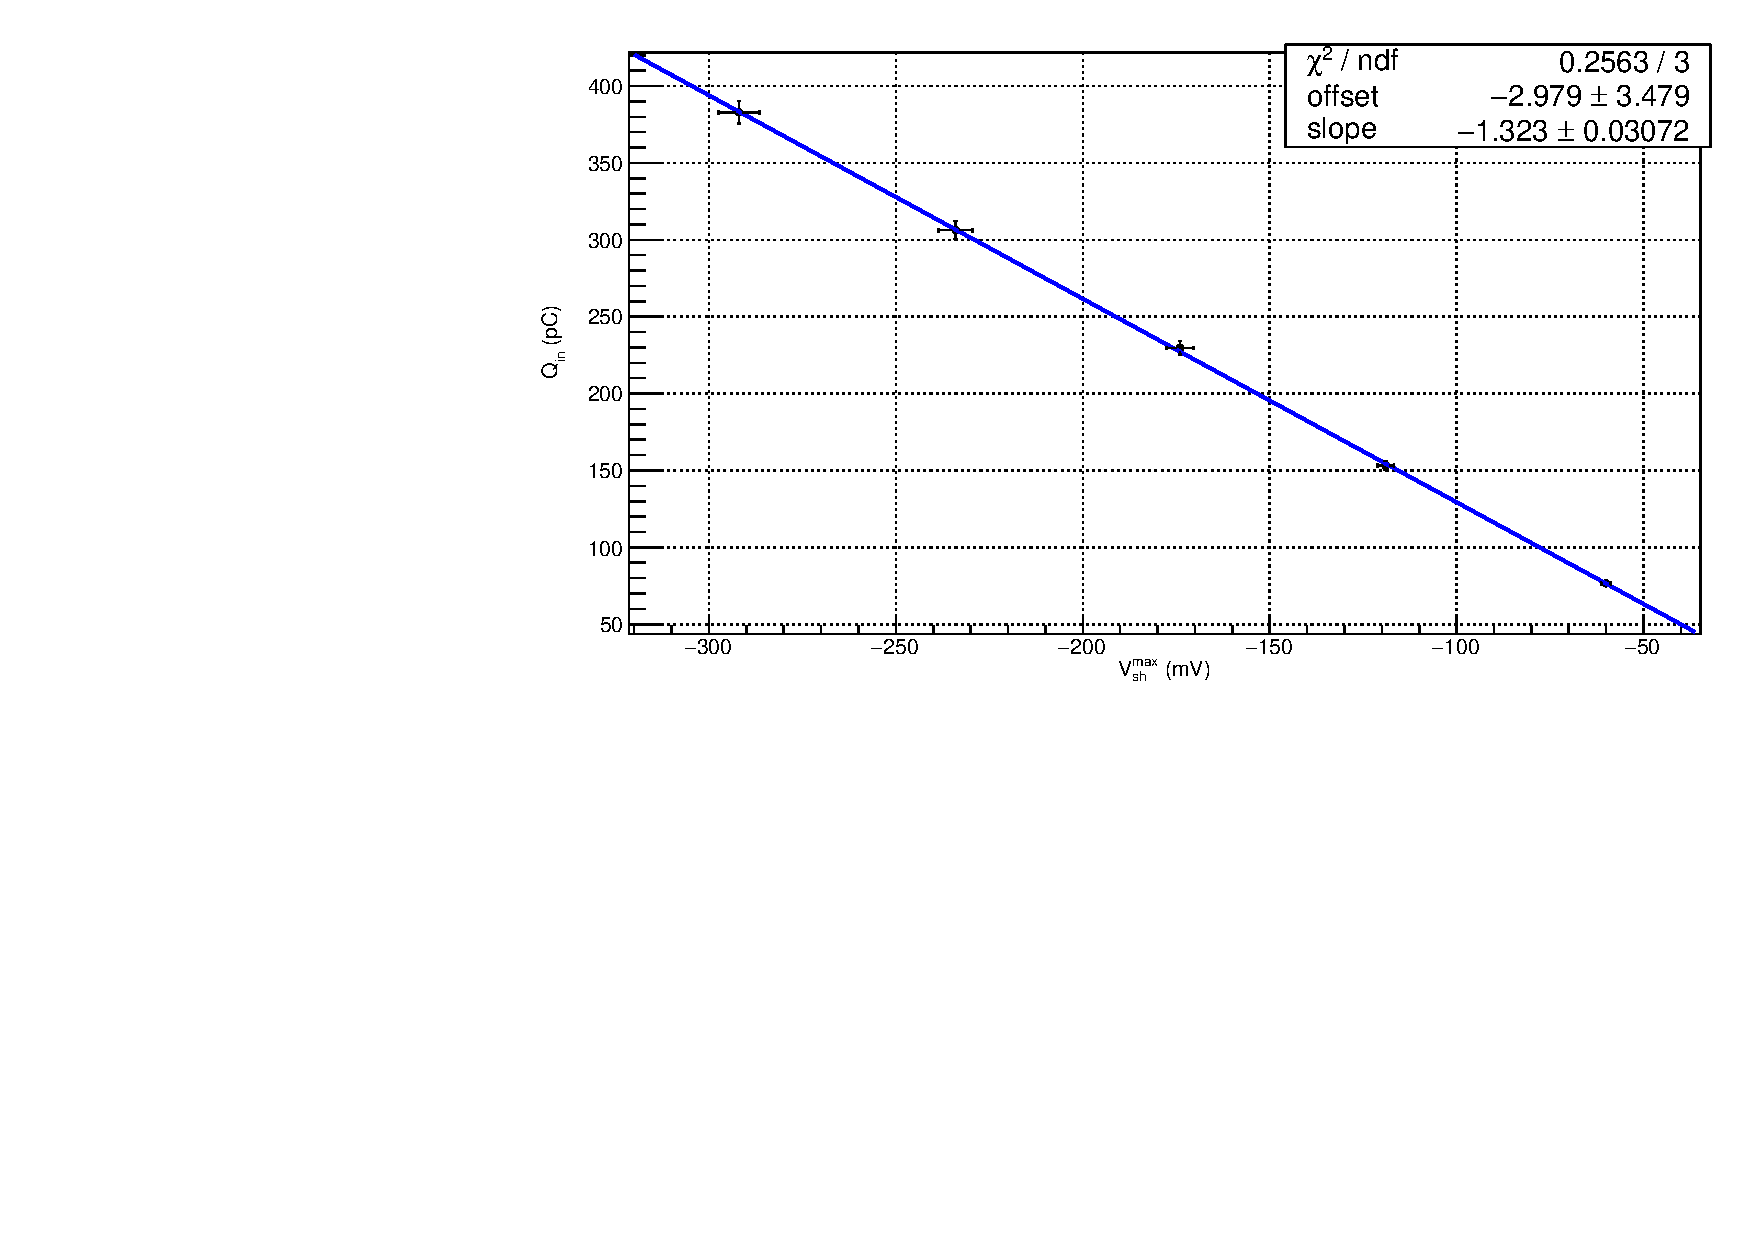
\includegraphics[scale=0.375, angle=0]{fitshaper.pdf}
    \caption{Carica iniettata e picco di tensione in uscita}
    \label{fig:fitshaper}
    \end{figure}
\end{center}

Segue il grafico dei residui

\begin{center}
    \begin{figure}[H]
    \centering
    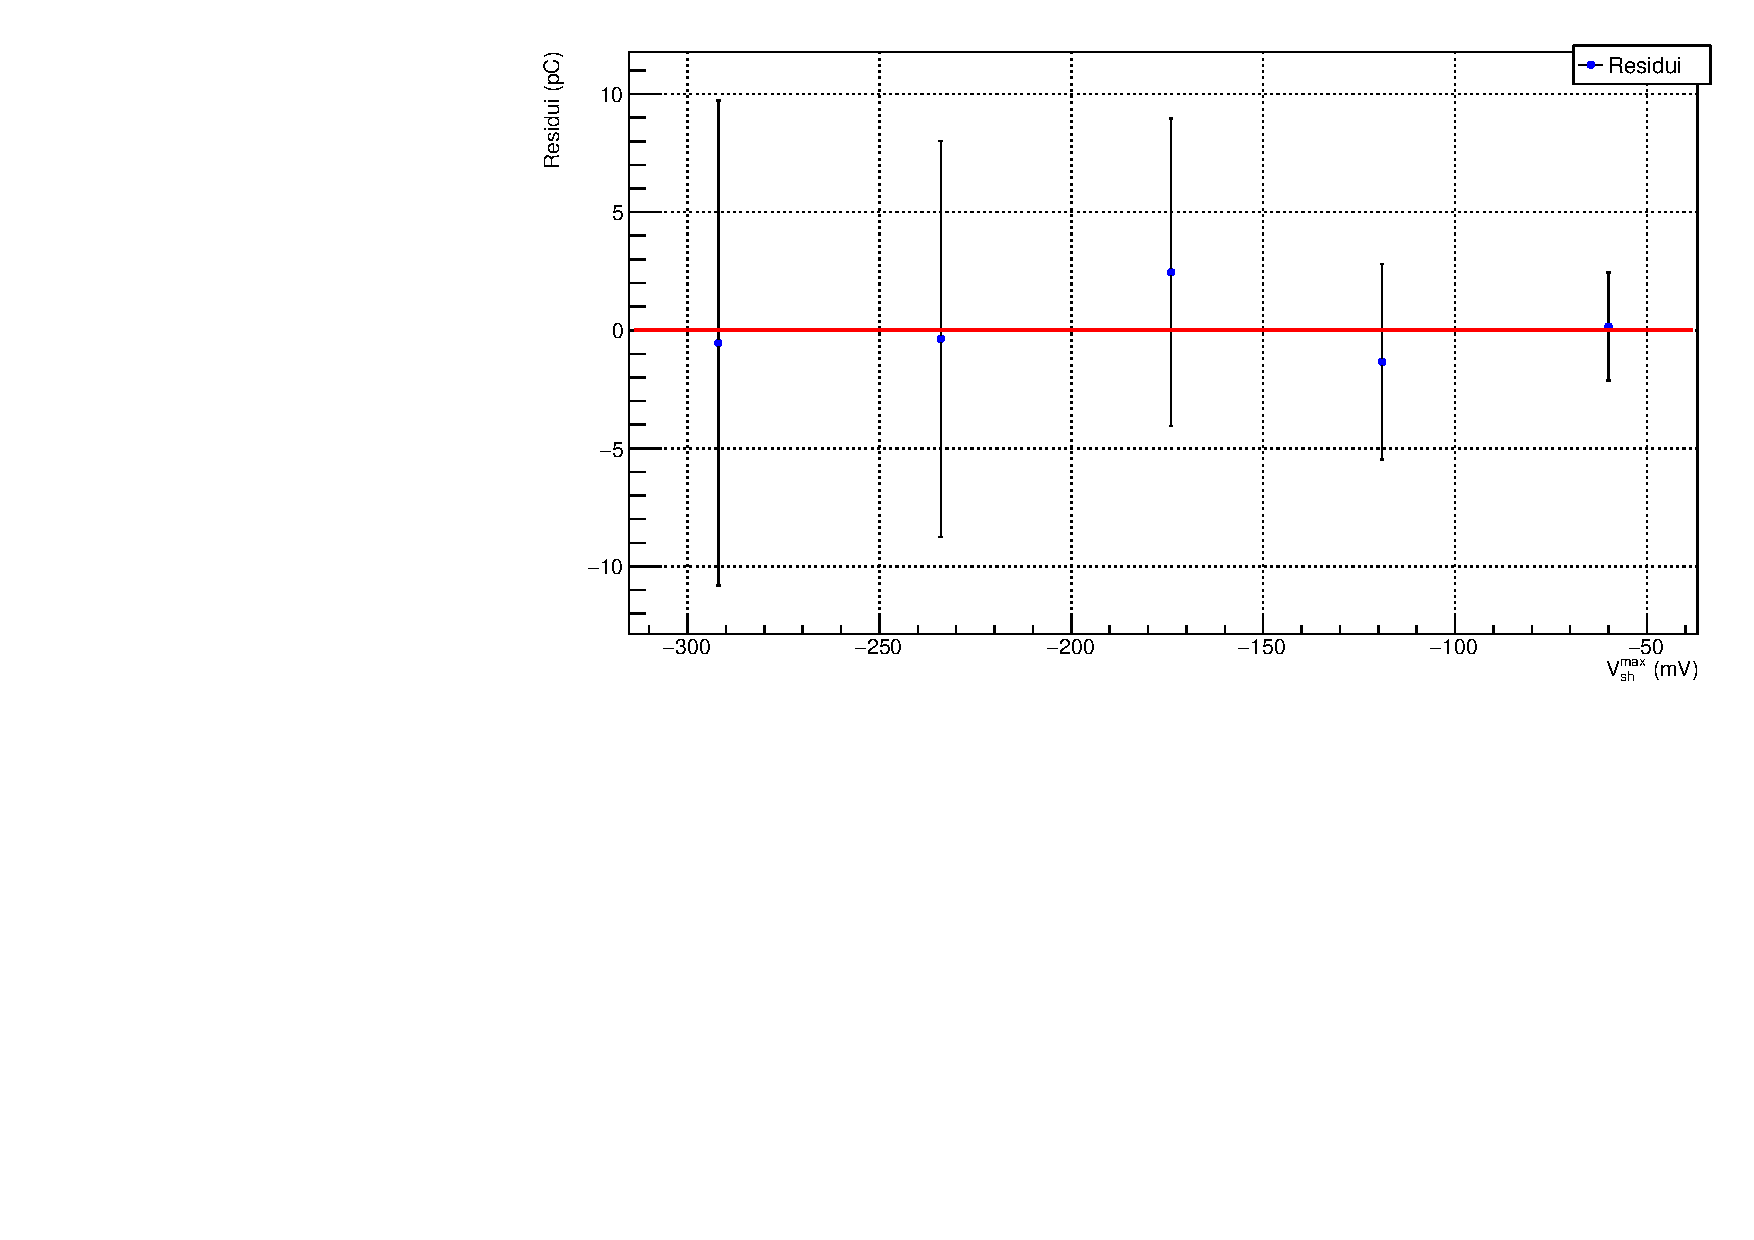
\includegraphics[scale=0.375, angle=0]{residuishaper.pdf}
    \caption{Grafico dei residui della relazione tra $Q_{in}$ e $V_{pre}^{max}$}
    \label{fig:residuishaper}
    \end{figure}
\end{center}

e i principali estimatori di bontà del fit.

\begin{table}[ht]
    \centering
    \begin{tabular}{ccccc}
        \toprule
        $\sigma_{y, post}$    &$\chi^{(2)}$    &$\lambda_{\chi}$   &$\rho$  &t   \\
        \midrule
        1.7 V               &0.26            &1.12              &-0.99993&-146.28\\
        \bottomrule
    \end{tabular}
    \caption{parametri di verifica della bontà del fit}
\end{table}

I parametri confermano la buona riuscita del fit lineare e dunque costituiscono la prova della relazione lineare che intercorre tra
carica iniettata e uscita dello shaper.

\section{Catena elettronica}

\subsection{Descrizione del circuito}

Unendo il circuto preamplificatore con il circuito formatore otteniamo un segnale correttamente processato ma negativo e dunque non
adatto all'acquisizione da parte di Arduino. Pertanto implementiamo un circuito amplificatore invertente, in particolare un
amplificatore di strumentazione. Tale apparato consiste di un opamp alimentato nell'ingresso invertente, capace dunque di cambiare
segno al segnale, preceduto da un buffer, che ha la funzione di garantire un'alta impedenza di ingresso: infatti con il solo 
amplificatore invertente il segnale cadrebbe sulla resistenza $R_{1a}$, mentre grazie alla presenza dell'inseguitore di tensione 
l'impedenza di ingresso è l'impedenza interna dell'opamp $U_1$, che si può considerare infinita.

Da semplici considerazioni si trova che la funzione di trasferimento è costante rispetto alla frequenza e data dal

\begin{equation}
    \label{eqn:ampinv_trasf}
    H = - \frac{R_{2a}}{R_{1a}} \left( \frac{R_{4a}}{R_{3a}} + 1 \right)
\end{equation}

Innanzitutto si è predisposta la corretta amplificazione, per poter visualizzare segnali dell'ordine di qualche volt immettendo
nel circuito impulsi della durata di qualche unità di $\mu s$: si deve dunque considerare la quantità di carica $Q_{in}$ 
scegliendo un impulso di durata $10 \mu s$ in ingresso, misurare l'uscita dell'apparato preamplificatore + shaper $V_{sh}$ 
e si calcola l'opportuno apparato resistivo in modo da generare in uscita un segnale di approssimativamente 2 V, cioè imporre, usando
la \ref{eqn:ampinv}, H = 2 V/$V_{sh}$, dove $V_{sh}$ corrisponde al picco in uscita dal formatore.

Variando poi la durata dell'impulso di $V_{in}$ e quindi la carica $Q_{in}$ è verificata la relazione lineare che ancora
intercorre con il $V_{out}$ della catena completa.

Introducendo poi segnali sinusoidali in ingresso di frequenza variabile si è effettuato un grafico di Bode per verificare la risposta
in frequenza della catena elettronica. Combinando quindi le funzioni di trasferimento del circuito preamplificatore 
\ref{eqn:preamp_trasf}, dello shaper compensato AGGIUNGERE RIFERIMENTO CORRETTA e dell'amplificatore di strumentazione 
\ref{eqn:ampinv_trasf}, si ottiene la funzione di trasferimento totale.

\begin{multline}
    \label{eqn:catena_trasf}
    |H(\omega)| = \frac{R_{pre}}{R_{in}} \frac{1}{\sqrt{1+\omega^2\tau_{pre}^2}} \cdot \\
    \cdot \frac{R_{sh}^2 + \omega^2 R_{pz}^2 \tau_{sh}^2}{(R_{sh}+R_{pz})^2 + \omega^2 R_{pz}^2 \tau_{sh}^2} \cdot \\
    \cdot \frac{R_{2a}}{R_{1a}} \left( \frac{R_{4a}}{R_{3a}} + 1 \right)
\end{multline}

\subsection{Discussione dati}

Utilizzando quindi il circuito fin qui costruito e iniettando la $V_{in}$ di cui sopra si trova $V_{sh} = (-282 \pm 5) mV$, pertanto
$H_{th} \approx 7$. Si può dunque scegliere le resistenze di conseguenza, in particolare:

\begin{align*}
    R_{1a} = (15.003 \pm 0.007) k\Omega \quad \sigma_{\%} = 0.05\% \\
    R_{2a} = (32.57 \pm 0.01) k\Omega \quad \sigma_{\%} = 0.04\% \\
    R_{1a} = (14.999 \pm 0.007) k\Omega \quad \sigma_{\%} = 0.05\% \\
    R_{1a} = (32.60 \pm 0.01) k\Omega \quad \sigma_{\%} = 0.04\% \\
\end{align*}

da cui $H_{sper}=-6.88$. Realizzato dunque il circuito si è proceduto con l'acquisizione di $V_{out}$ al variare dell'impulso in
ingresso, di cui si riportano di seguito dati e fit lineare.

\begin{center}
\begin{figure}[H]
\centering
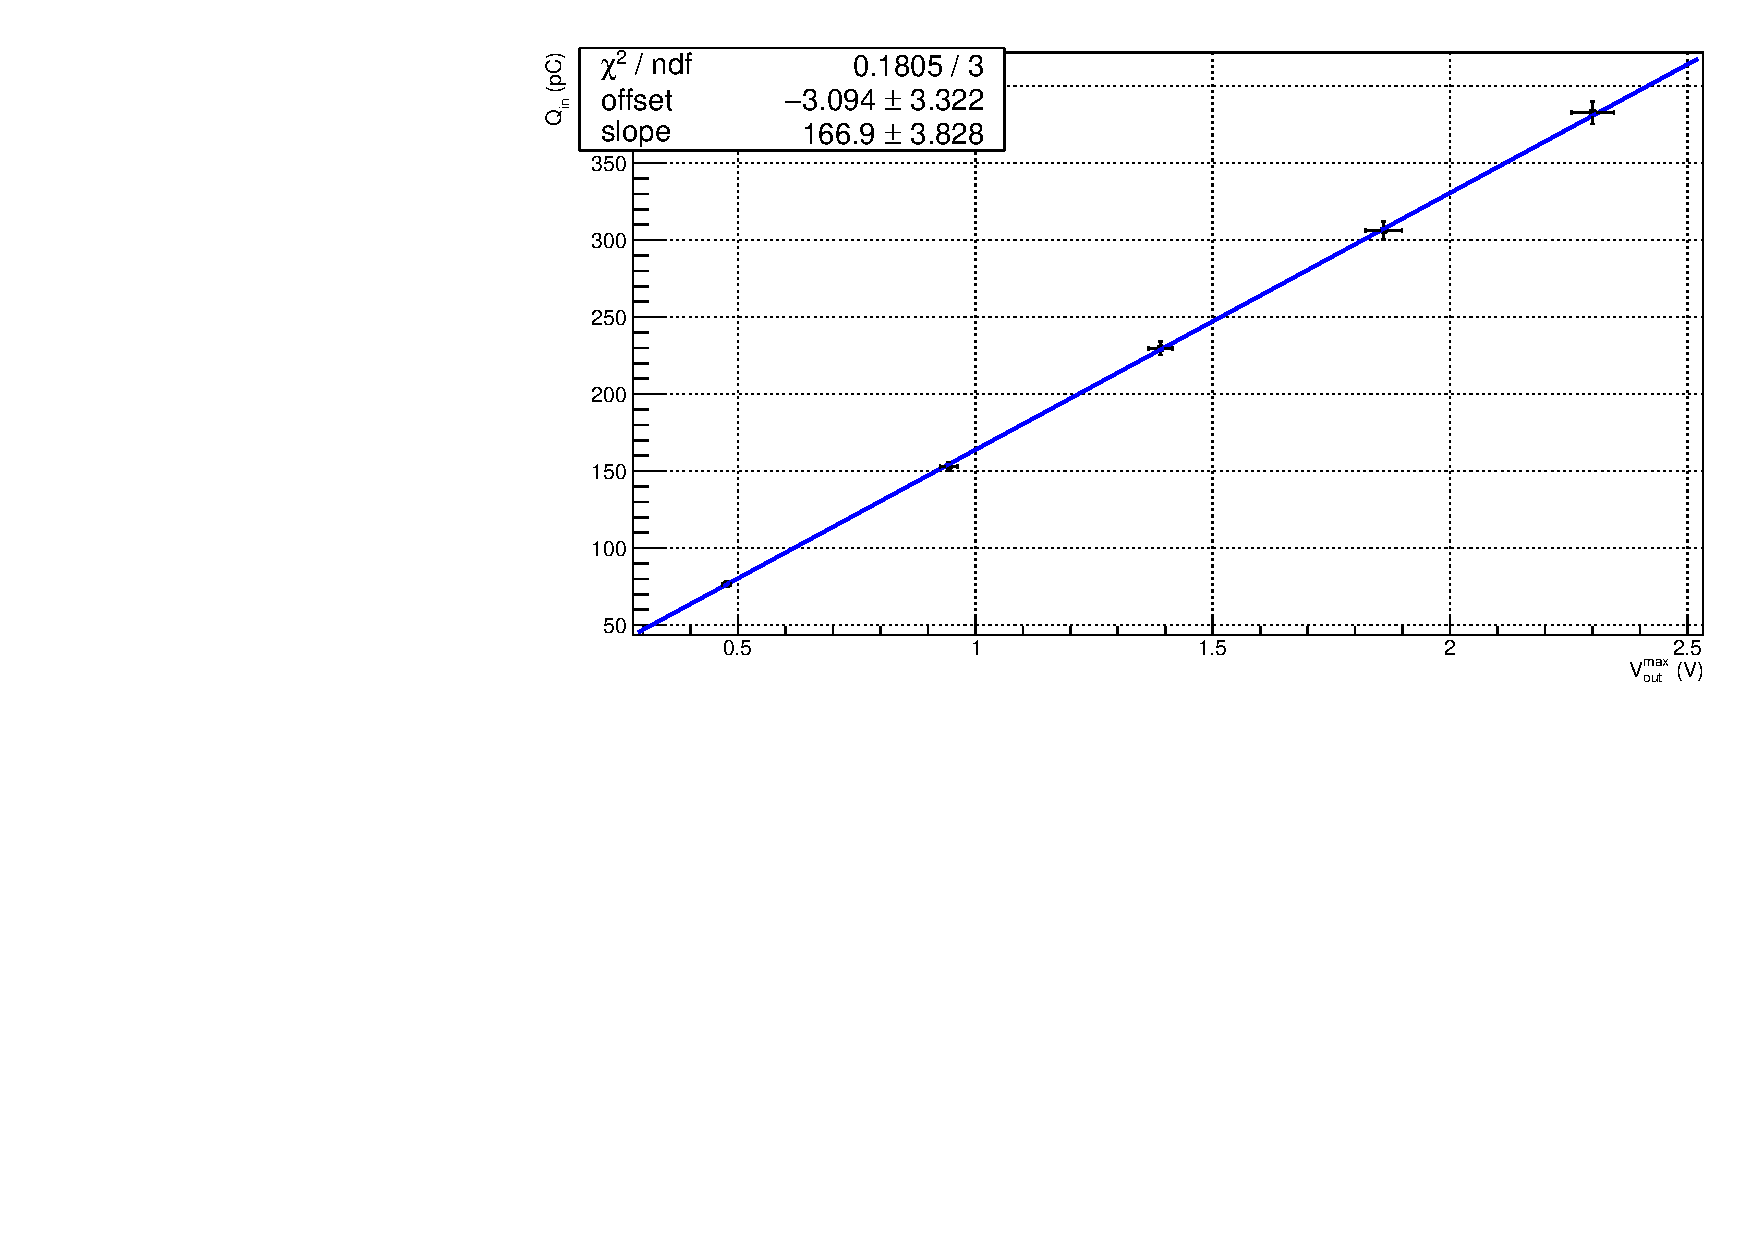
\includegraphics[scale=0.4, angle=0]{fitcatena.pdf}
\caption{Relazione lineare tra carica iniettata e uscita della catena}
\label{fig:catenaQvsV}
\end{figure}
\end{center}

\begin{center}
\begin{figure}[H]
\centering
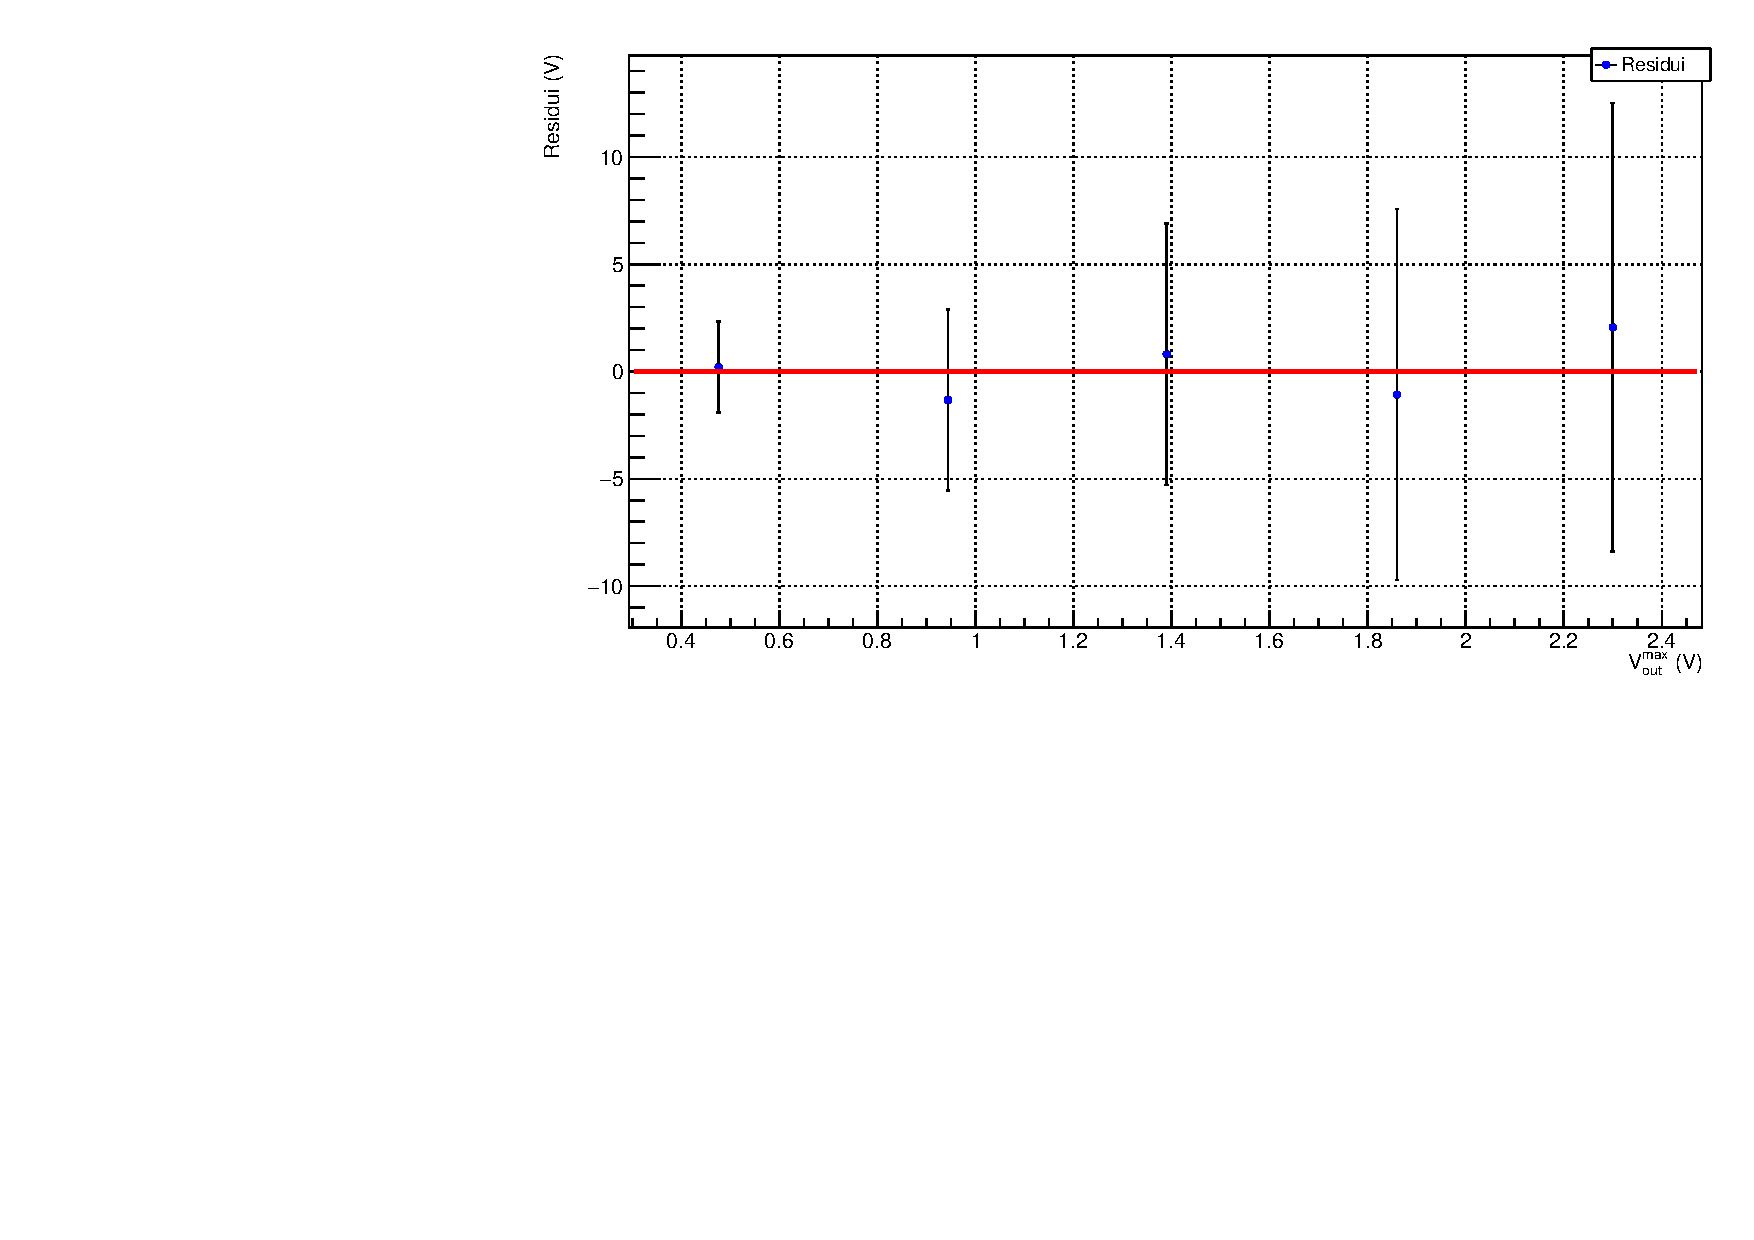
\includegraphics[scale=0.4, angle=0]{residuicatena.pdf}
\caption{Grafico dei residui della relazione tra $Q_{in}$ e $V_{out}$}
\label{fig:catenaQvsV_res}
\end{figure}
\end{center}

\begin{table}[ht]
    \centering
    \begin{tabular}{ccccc}
        \toprule
        $\sigma_{y, post}$    &$\chi^{(2)}$    &$\lambda_{\chi}$   &$\rho$ &t   \\
        \midrule
        1.6 pC                &0.18            &1.15               &0.99994&167.63\\
        \bottomrule
    \end{tabular}
    \caption{parametri di verifica della bontà del fit}
\end{table}

Si osserva che i parametri di bontà del fit sono buoni, a testimonianza di una ben verificata relazione

Successivamente si presenta il grafico di Bode della catena, in cui sono raffigurati i dati sperimentali, i dati simulati
su LTspice e il modello teorico espresso dalla \ref{eqn:catena_trasf}.

\begin{center}
\begin{figure}[H]
\centering
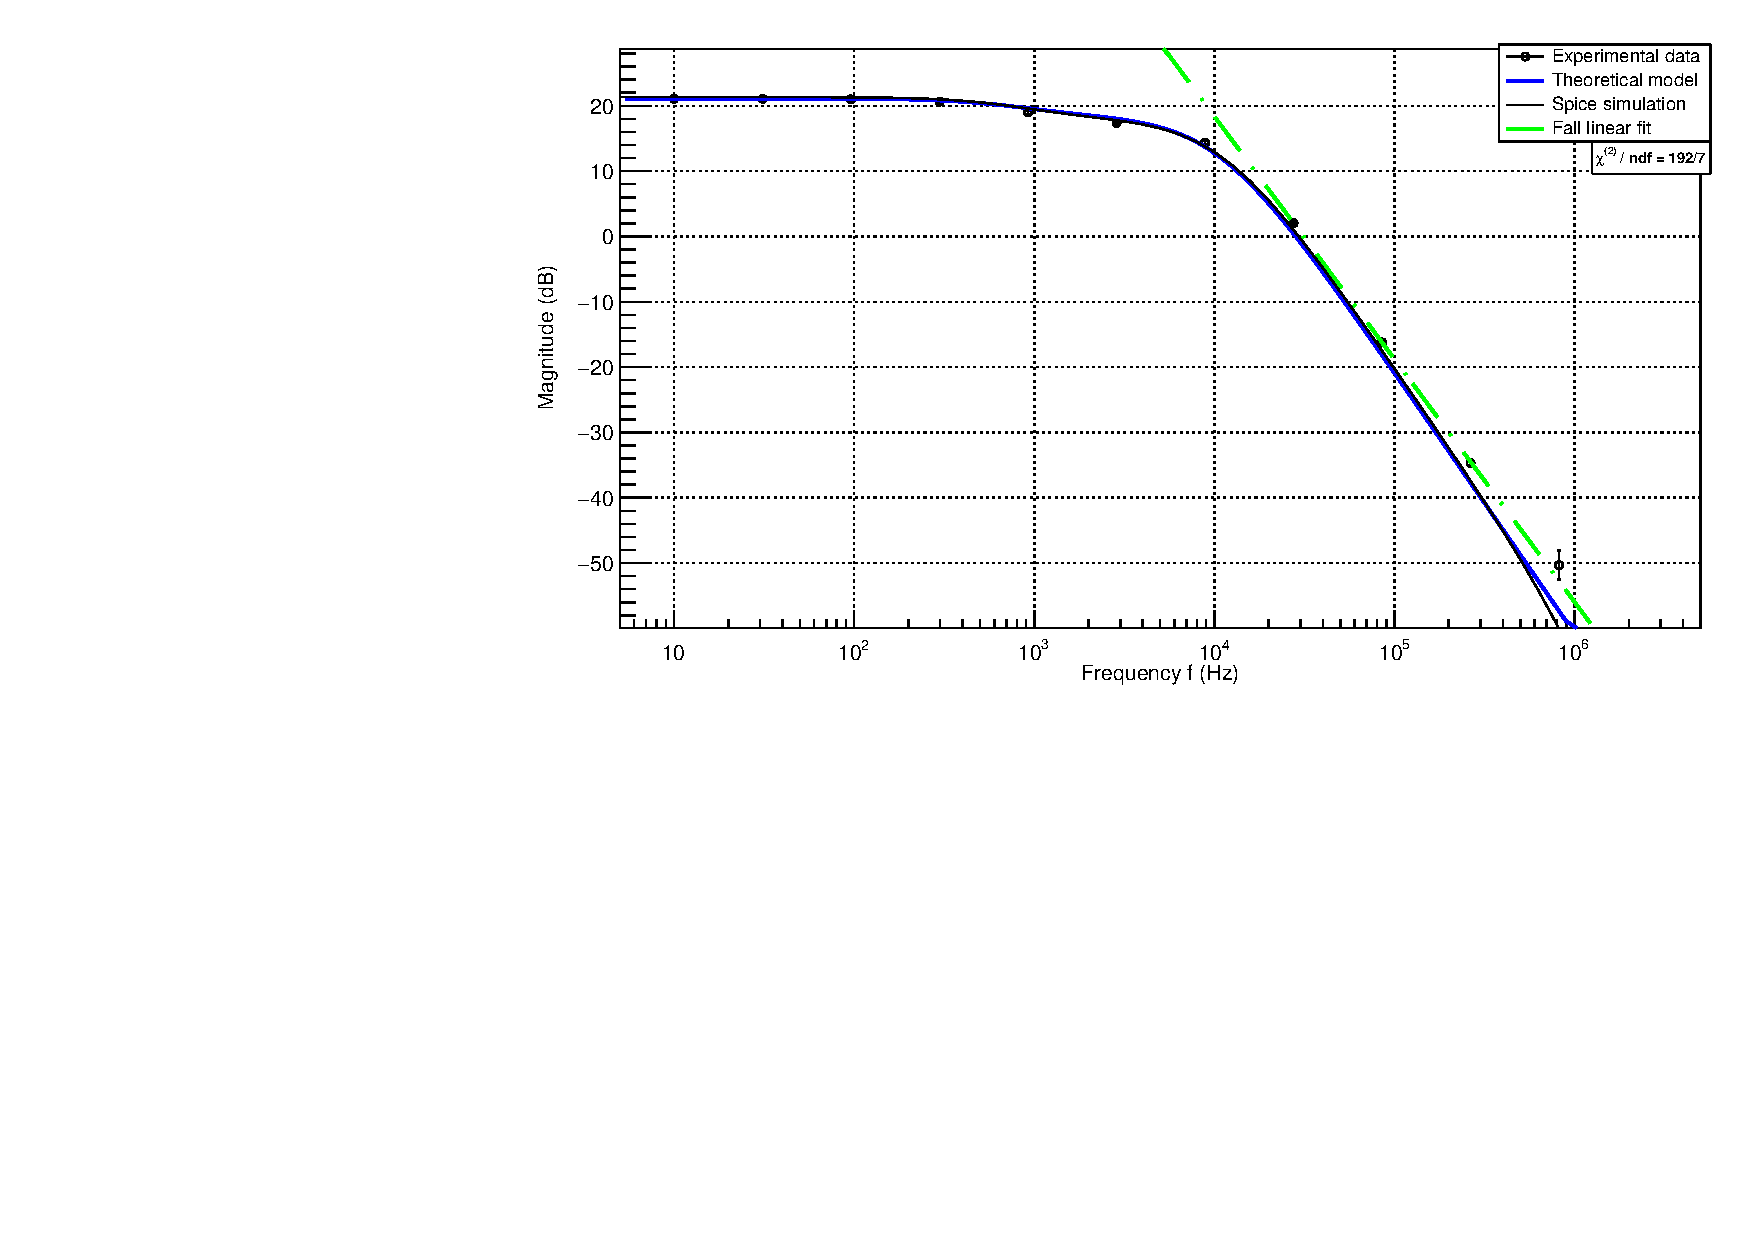
\includegraphics[scale=0.4, angle=0]{bodecatena.pdf}
\caption{Grafico di Bode della risposta in frequenza della catena elettronica}
\label{fig:catenaQvsV}
\end{figure}
\end{center}

\begin{center}
\begin{figure}[H]
\centering
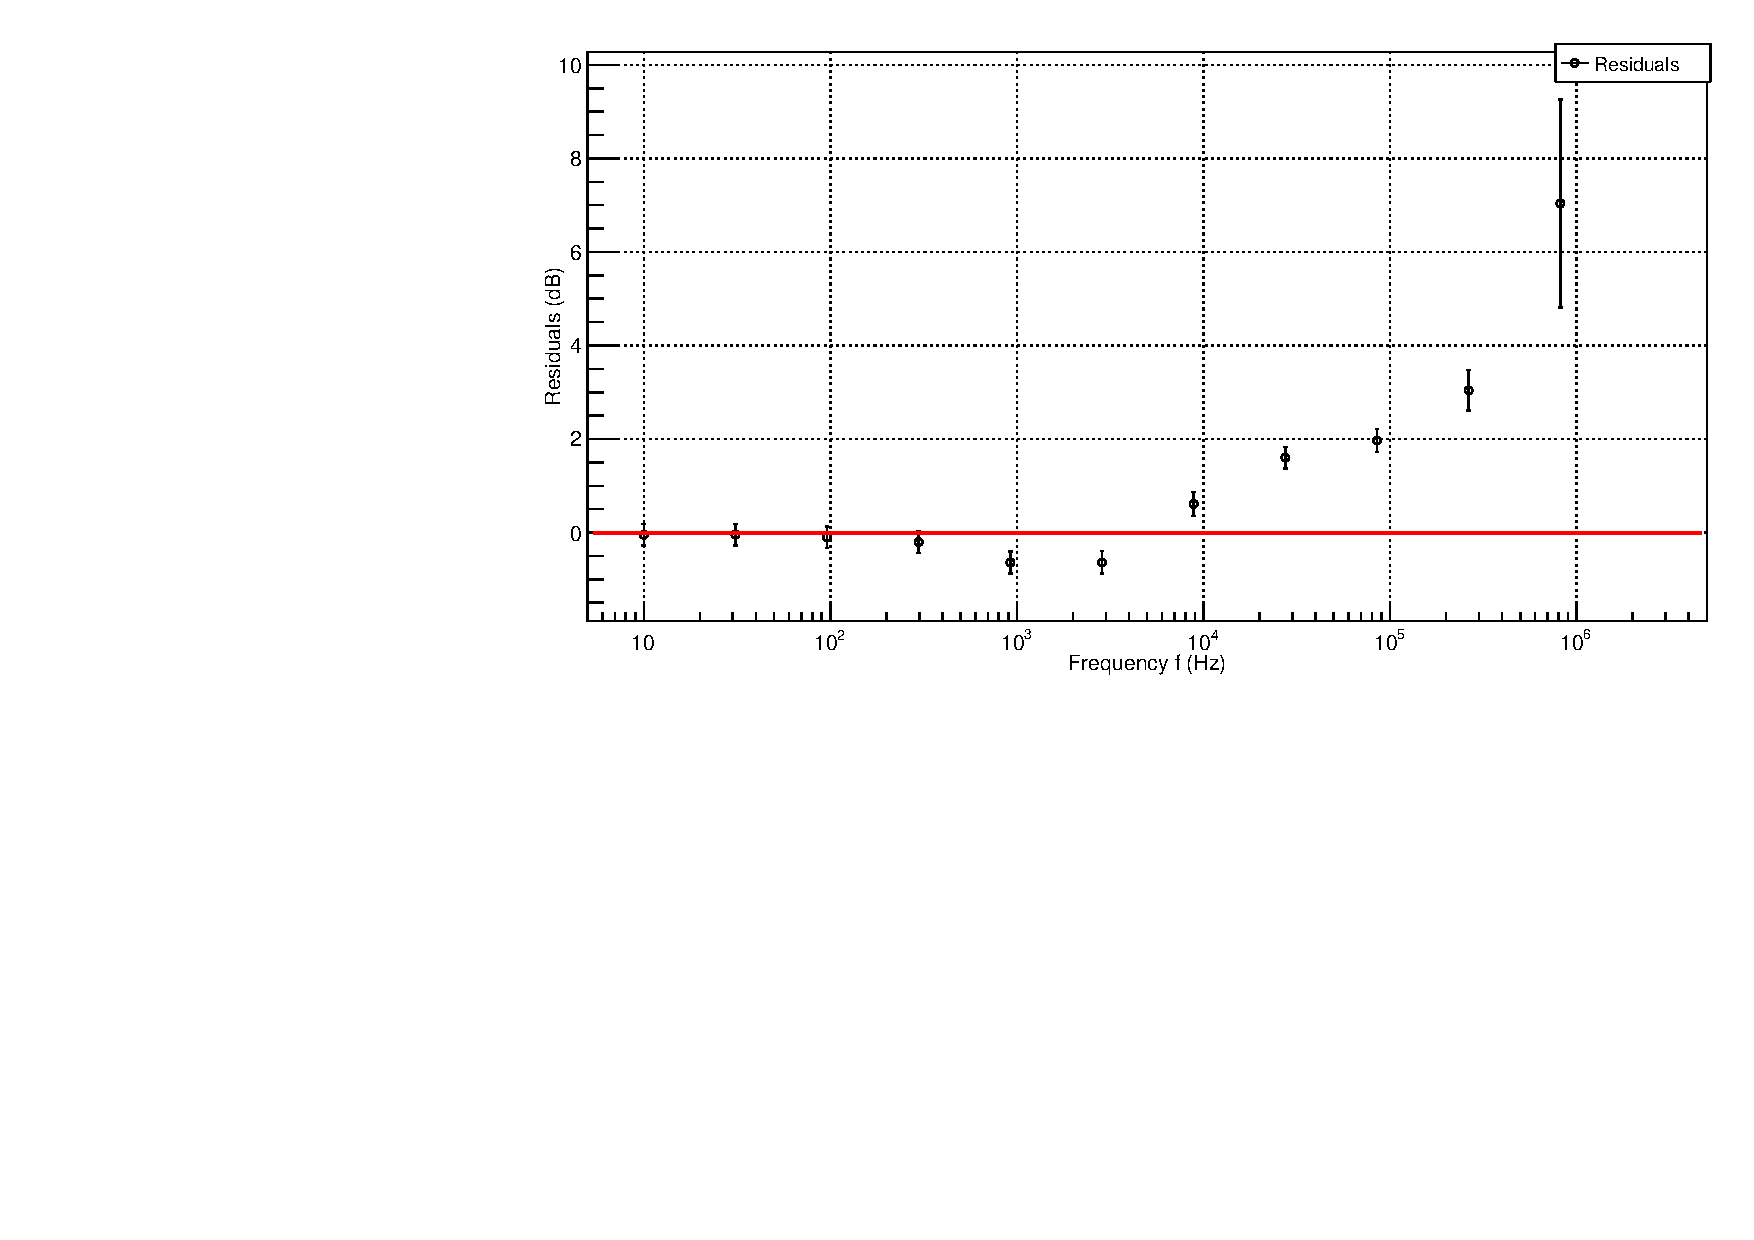
\includegraphics[scale=0.4, angle=0]{bodecatenaresidui.pdf}
\caption{Grafico dei residui tra dati sperimentali e modello}
\label{fig:catenaQvsV_res}
\end{figure}
\end{center}

Dal grafico dei residui si può osservare un certa incompatibilità dei dati, imputabile a una sottostima degli errori? 

\section{Acquisizione forme d'onda con Arduino}

Ora la catena elettronica restituisce un segnale correttamente processato e amplificato, adatto alla rivelazione da parte di una scheda Arduino Due. Prima di iniziare
l'acquisizione delle forme d'onda restituite dal circuito, occorre comprendere la taratura della scheda per poi gestire i dati sperimentali. Si effettuano dunque delle 
acquisizioni preliminari al fine di realizzare una calibrazione orizzontale (sui tempi) e una verticale (sulle tensioni).

In particolare per la calibrazione orizzontale si sono utilizzate onde sinusoidali di diversa frequenza (e dunque periodo), confrontando
il periodo T con il conteggio dei punti nell'acquisizione secondo la formula $T = a + b \cdot ch$, dove ch rappresenta il periodo in 
counts stimato attraverso un algoritmo che individua punti di massimo e di minimo successivi nella forma sinusoidale.

\begin{center}
\begin{figure}[H]
\centering
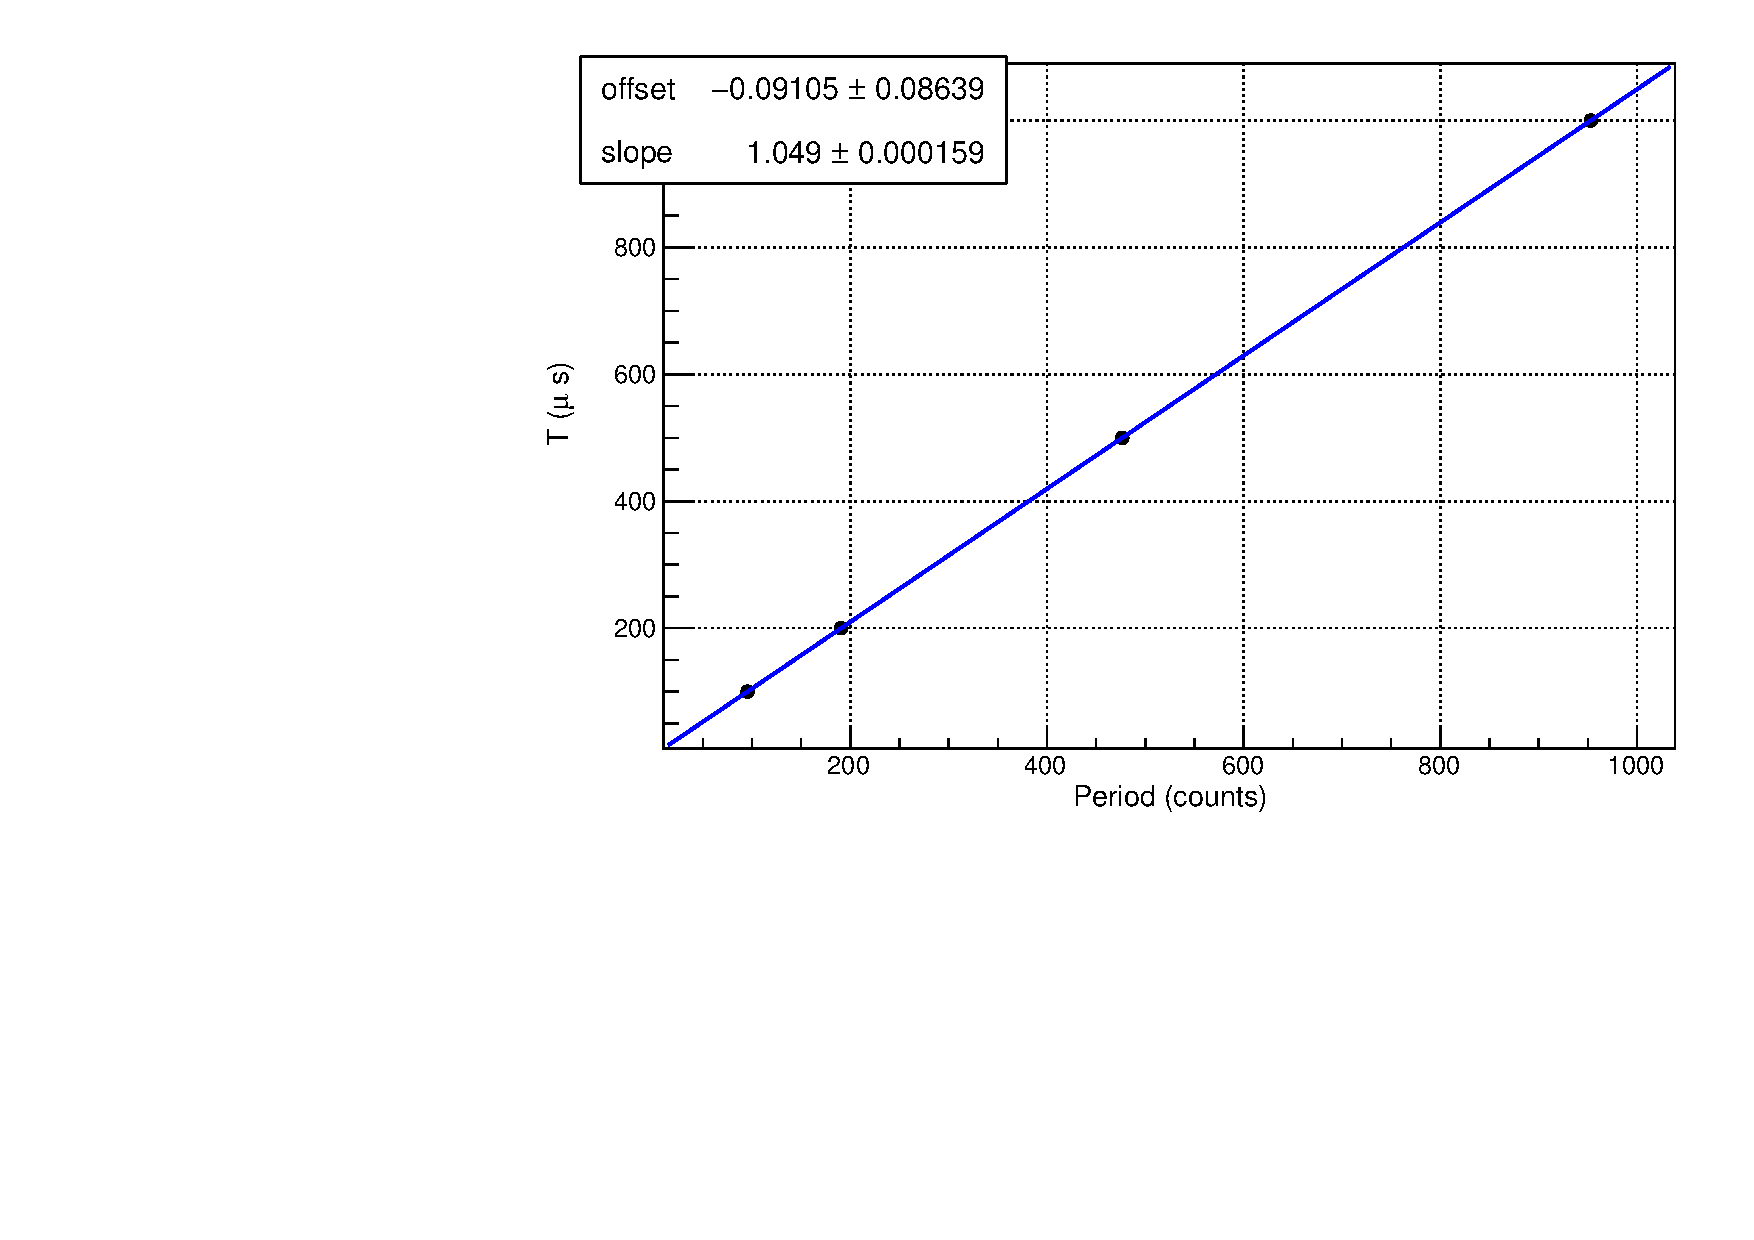
\includegraphics[scale=0.4, angle=0]{calibtempi.pdf}
\caption{Calibrazione temporale}
\label{fig:calibtempi}
\end{figure}
\end{center}

\begin{center}
\begin{figure}[H]
\centering
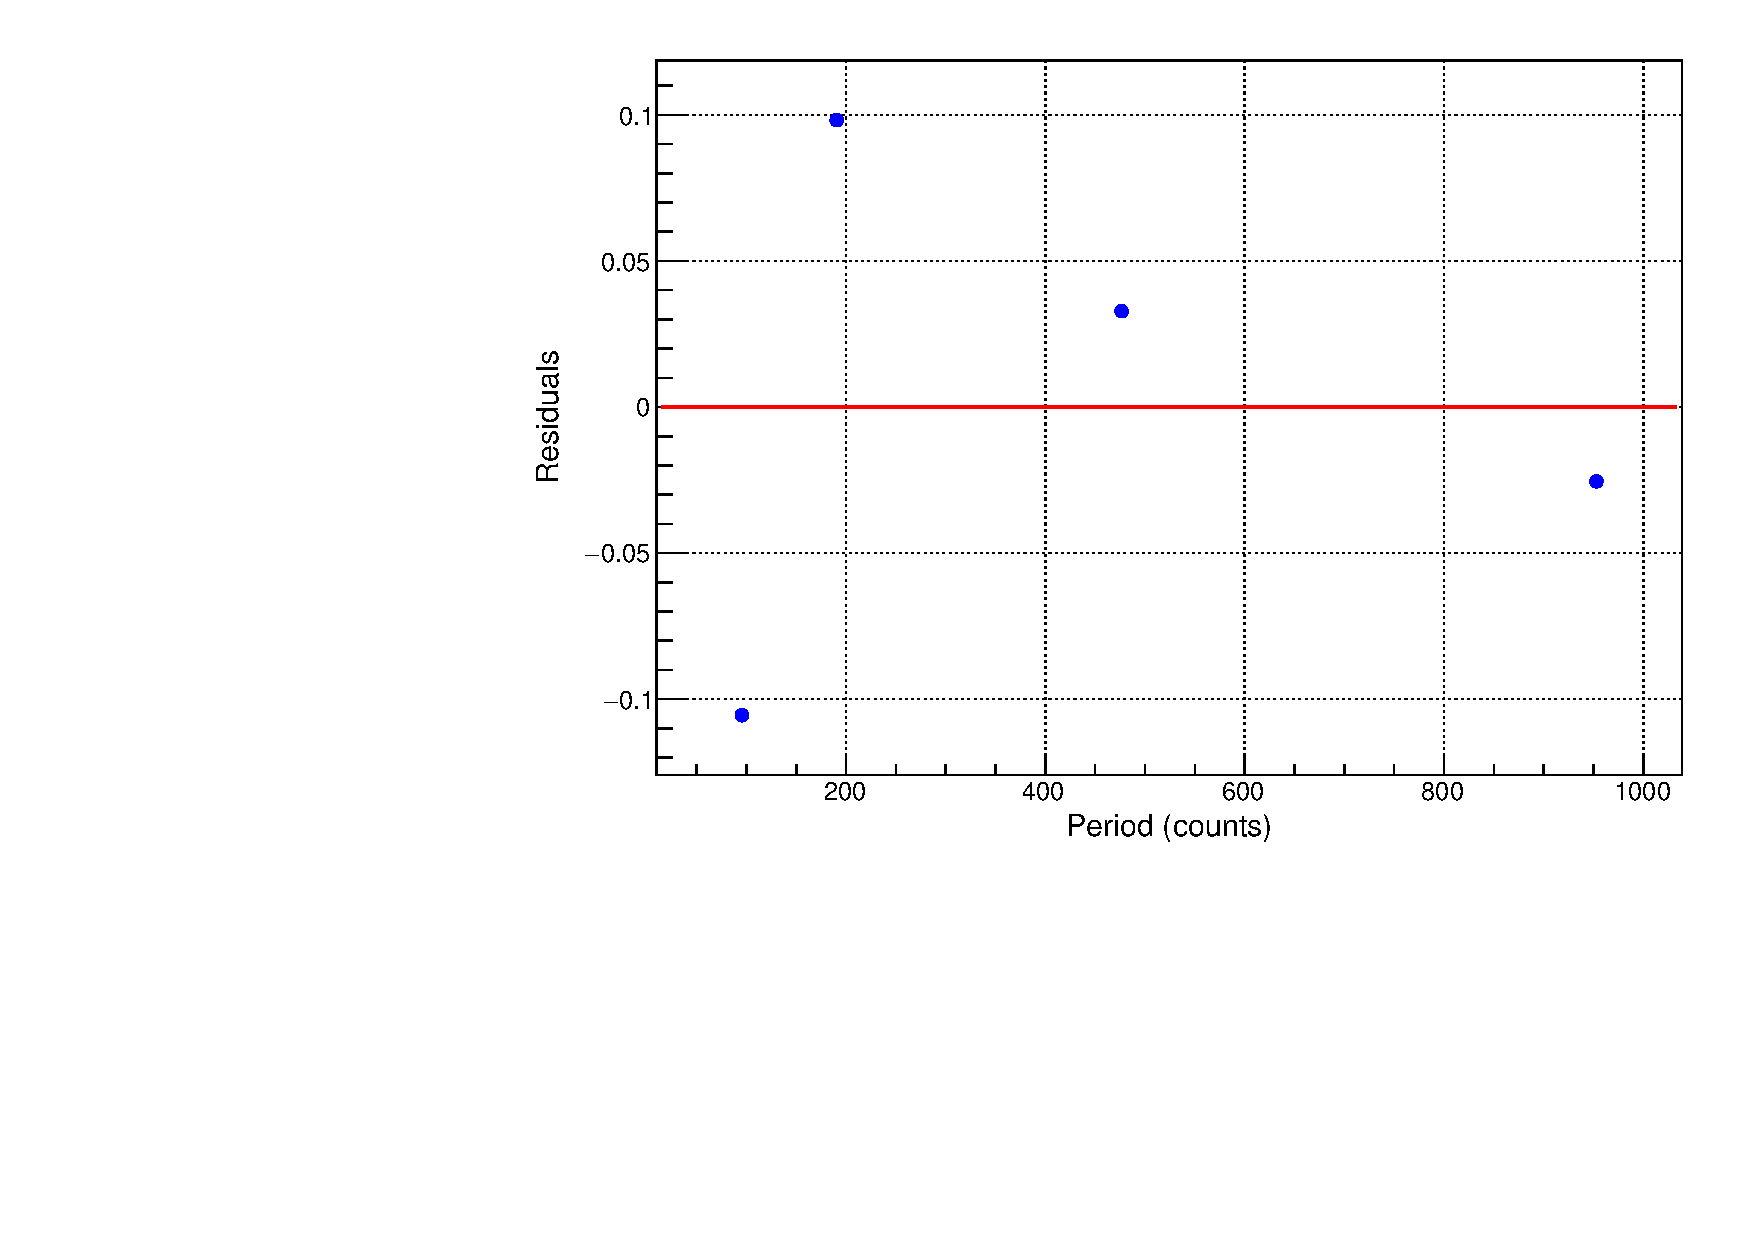
\includegraphics[scale=0.4, angle=0]{calibtempiresidui.pdf}
\caption{Residui del fit di calibrazione temporale}
\label{fig:calibtempiresidui}
\end{figure}
\end{center}

Ne si ricava che il software acquisisce un punto in ogni intervallo pari alla slope b, ossia ogni $(1.0490 \pm 0.0002)\mu s$.

Per la calibrazione verticale sulle tensioni si sono immesse nel circuito onde quadrate tra 0 e una tensione di altezza variabile, 
per poi effettuare nuovamente un fit lineare del tipo $V = a + b \cdot ch$, dove ch stavolta esprime il plateau della tensione 
in conteggi: il parametro b fornirà il fattore di conversione mV/counts, mentre a rappresenterà l'offset aggiunto dalla scheda al 
segnale letto.

\begin{center}
\begin{figure}[H]
\centering
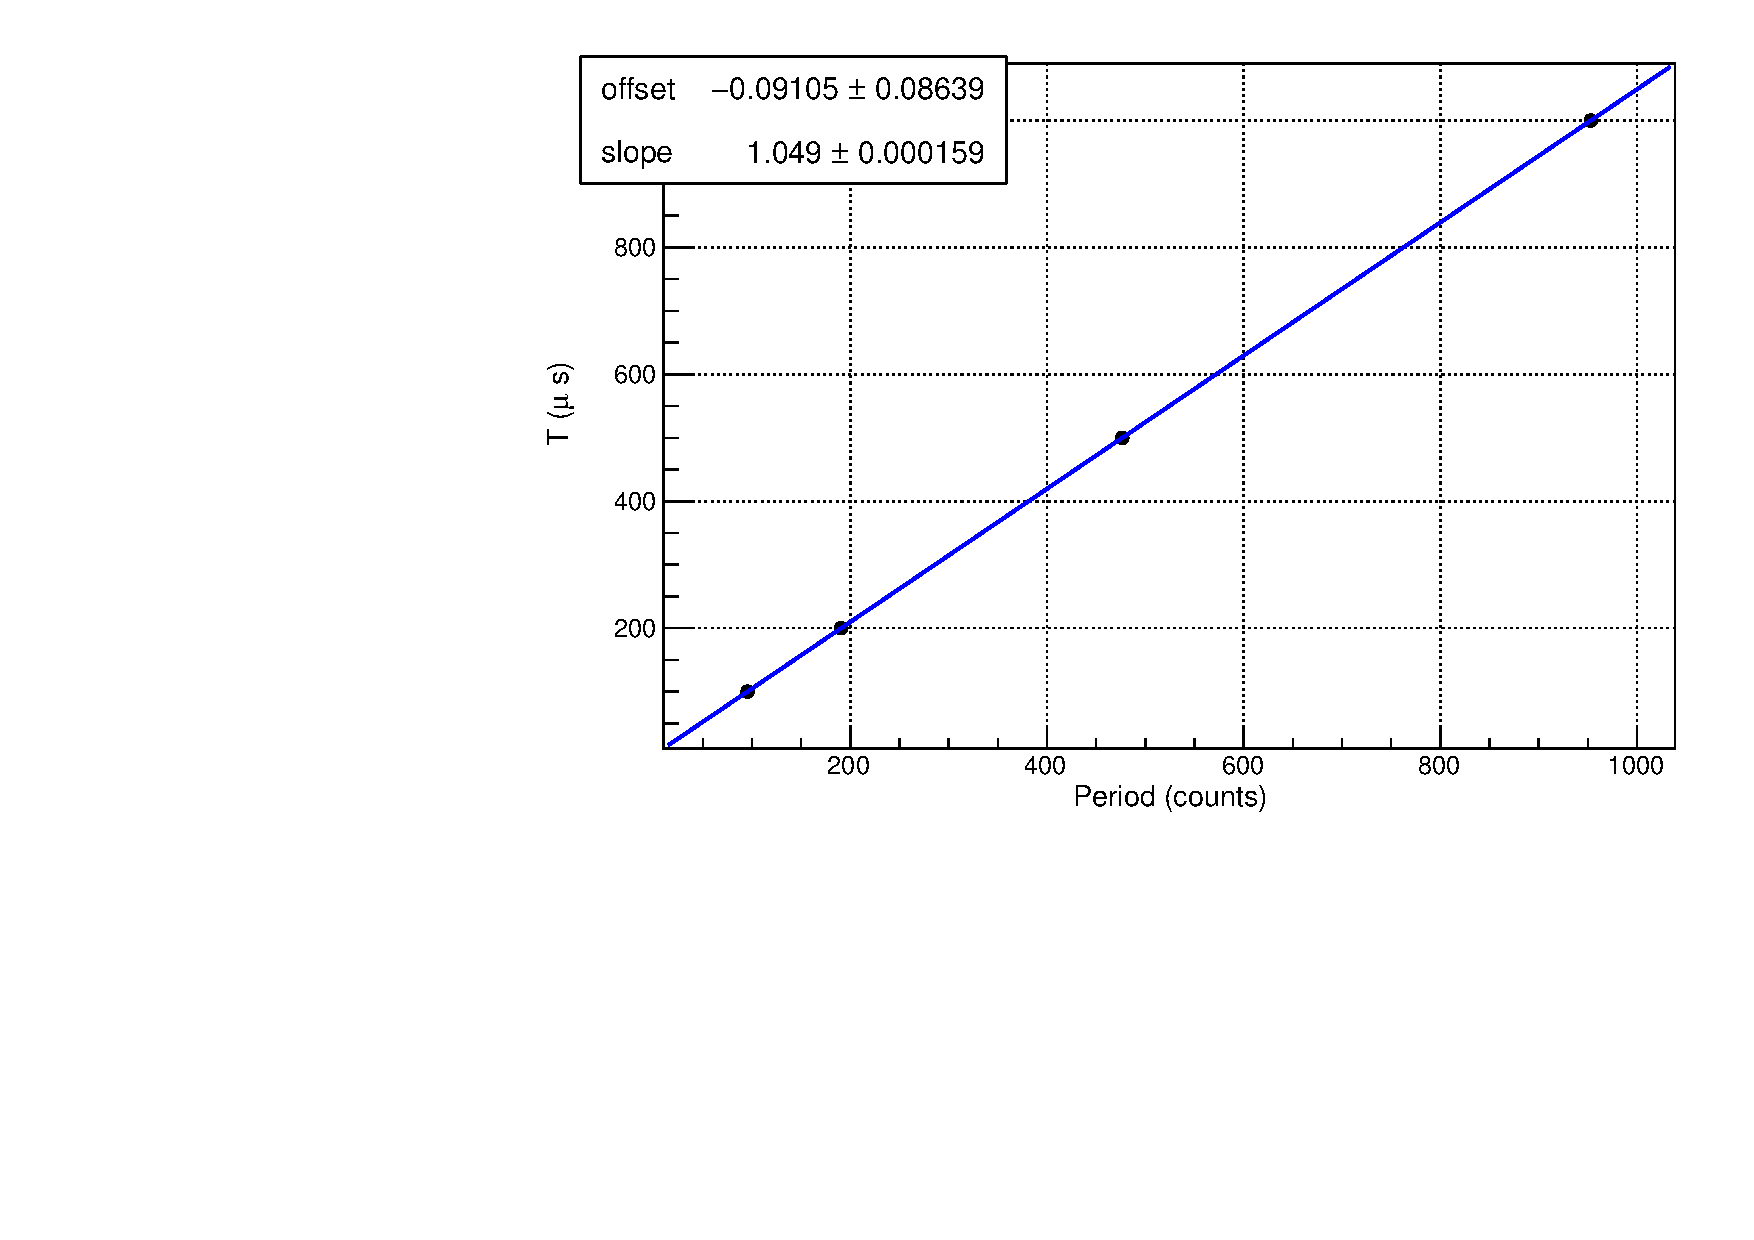
\includegraphics[scale=0.4, angle=0]{calibtempi.pdf}
\caption{Calibrazione temporale}
\label{fig:calibtempi}
\end{figure}
\end{center}

\begin{center}
\begin{figure}[H]
\centering
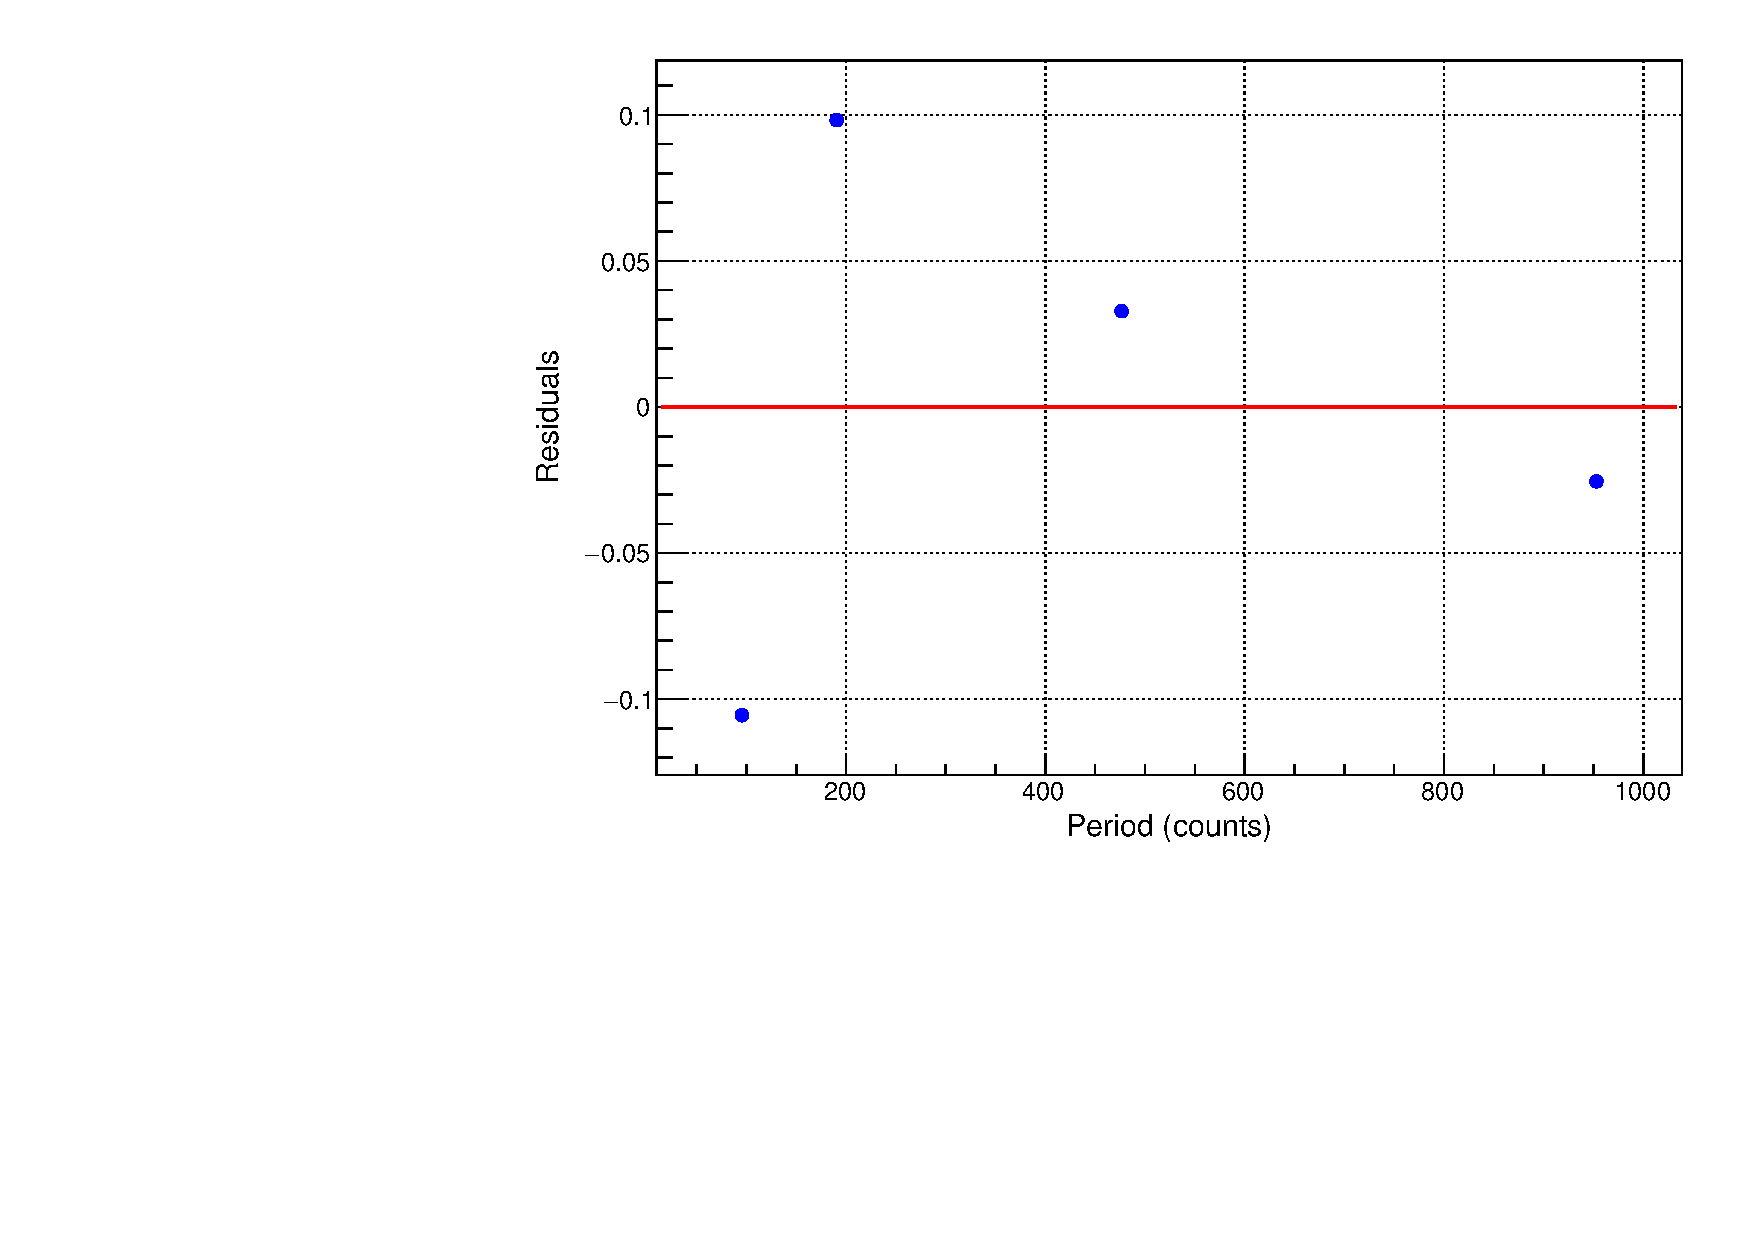
\includegraphics[scale=0.4, angle=0]{calibtempiresidui.pdf}
\caption{Residui del fit di calibrazione temporale}
\label{fig:calibtempiresidui}
\end{figure}
\end{center}


Effettuata dunque la calibrazione, si è acquisita la forma d'onda in uscita dalla catena elettronica completa con in input il solito
impulso di tensione, partendo da una durata di $10 \mu s$ e diminuendola via via di un'unità ad ogni nuova acquisizione.



\section{Conclusioni}

\appendix
\section{Appendici}
\label{appendice}
\subsection{Costruzione dell'errore sulle misure}
\label{Calcerr}

Nel trattare i dati rilevati dall'oscilloscopio nel corso dell'esperienza si sono assegnati gli errori alle misure tenendo conto che ogni misura è affetta da un'incertezza di origine sistematica e da una di lettura, dovuta al posizionamento dei cursori sulla schermata. Per semplificare il calcolo degli errori, si sceglie di considerare un errore massimo $\Delta_{\%}$ di tipo percentuale per identificare il contributo sistematico presente nella presa dati, e un errore massimo $\Delta_{lett}$ per coprire le fluttuazioni casuali. La percentuale del valore letto da utilizzare come $\Delta_{\%}$ è del $3\%$ per le tensioni e dello $0.01\%$ sui tempi: per quanto riguarda invece l'errore di lettura, si è considerato 1/10 della divisione utilizzata.
Tuttavia, poiché l'errore percentuale sui tempi è sempre decisamente trascurabile rispetto a quello di lettura, lo si è omesso nel calcolo dell'incertezza totale.

Infine, si precisa che tutti i risultati sono presentati con un errore non massimo, ma di tipo statistico: si riporta la regola di conversione, in ipotesi di distribuzione uniforme per l'errore sistematico e in ipotesi di distribuzione triangolare per l'errore di lettura.

\begin{equation}
\sigma_{\%}=\frac{2\Delta_{\%}}{\sqrt{12}} \quad \quad \sigma_{lett}=\frac{2\Delta_{lett}}{\sqrt{24}}
\end{equation}

Un meccanismo analogo vale per le misure dirette di grandezze quali resistenze e capacità effettuate con il multimetro: anche in questo caso abbiamo un contributo sistematico e uno casuale, il primo dato ancora da un errore percentuale e il secondo da un errore in digit. Tale contributo in digit è dato da $\Delta_{dgt}=ns$ dove $n=\#digit$ è un numero intero riportato sul manuale dello strumento e $s$ è la sensibilità usata nella lettura del valore. Anche qui si utilizza la conversione in errori statistici in ipotesi di distribuzione uniforme.

\subsection{Commento sull'accettazione/rifiuto dei fit}
Nel corso della relazione sono stati riportati diverse volte i parametri per la verifica della bontà del fit, sostenendo che essi permettessero di accettare o rifiutare l'interpolazione.


Per quanto riguarda i valori di $\chi^{(2)}$, l'ipotesi che il fit descriva i dati viene accettata o rifiutata con 0.90 CL, mentre
per il valore di $t$ di Student l'ipotesi di non correlazione è stata rifiutata o accettata con lo stesso CL.


\subsection{Tabella delle compatibilità}
\medskip
\begin{table}[H]
    \centering
    \begin{tabular}{c}
        %\hline
        \begin{Large}
        $\lambda=\frac{|a-b|}{\sqrt{\sigma_a^2+\sigma_b^2}}$
        \end{Large}\\
        %\hline
    \end{tabular}
    \hspace{0.5cm}
    \begin{tabular}{cc}
        \toprule
        &       \textbf{Compatibilità   }       \\
        \midrule
        0$\leq \lambda$<1   &Ottima                 \\
        1<$\leq \lambda$<2   &Buona                  \\
        2<$\leq \lambda$<3   &Accettabile            \\
        3<$\leq\lambda$<5   &Pessima                \\
        $ \lambda \geq $  5     &Non compatibile        \\
        \bottomrule
    \end{tabular}
    \caption{Indicazioni lettura compatibilità}
\end{table}

\subsection{Dati sperimentali}
\end{document}
